\documentclass[abstract, english]{scrartcl}
\addtokomafont{disposition}{\boldmath}

% LuaLatex
% \usepackage{polyglossia}
% \setmainlanguage{english}

% \usepackage{fontspec}
% \setmainfont[
%     Ligatures=TeX,
%     SmallCapsFont={Latin Modern Roman Caps},
%     SlantedFont={* Slanted},
%     ItalicFeatures  = {
%         SmallCapsFont = {LMRomanCaps10-Oblique}
%     },
%     ]{Latin Modern Roman}

% pdflatex
\usepackage[english]{babel}
\usepackage[T1]{fontenc}
\usepackage[utf8]{inputenc}
\usepackage{lmodern}

\usepackage{microtype}

\usepackage{todonotes}
\usepackage{blindtext}

\usepackage{amsmath}
\usepackage{amssymb}
\usepackage{mathdots}
\usepackage{mathtools}
\usepackage{csquotes}
\usepackage{enumitem}

\usepackage{subcaption}
\usepackage[font=small, labelfont=bf, format=hang, indention=-2em]{caption}

\usepackage{algorithm}
\usepackage[noend]{algpseudocode}

\usepackage[hyperref,thmmarks,amsmath]{ntheorem}

\usepackage{url}
\usepackage[pdftex, hypertexnames=false, unicode]{hyperref}
\usepackage[nameinlink, noabbrev]{cleveref}

\usepackage{tikz}
\usepackage{pgfplots}
\pgfplotsset{compat=1.12}
\usetikzlibrary{calc}

%%%

\theoremstyle{plain}
\theoremheaderfont{\rmfamily\bfseries\upshape\boldmath}
\theorembodyfont{\itshape}
\theoremseparator{}
\theoremsymbol{}
\newtheorem{definition}{Definition}
\newtheorem{theorem}[definition]{Theorem}
\newtheorem{lemma}[definition]{Lemma}
\newtheorem{problem}[definition]{Problem}
\newtheorem{observation}[definition]{Observation}

\theoremstyle{plain}
\theoremheaderfont{\scshape}
\theorembodyfont{}
\theoremseparator{}
\theoremsymbol{\qed}
\newtheorem*{proof}{Proof}

\theoremstyle{break}
\theoremheaderfont{\rmfamily\bfseries\upshape\boldmath}
\theorembodyfont{}
\theoremseparator{}
\theoremsymbol{}
\newtheorem{Algorithm}[definition]{Algorithm}

\crefname{observation}{observation}{observations}
\Crefname{observation}{Observation}{Observations}
\crefname{Algorithm}{algorithm}{algorithms}
\Crefname{Algorithm}{Algorithm}{Algorithms}

%%%

\newcommand{\R}{\mathbb{R}}
\newcommand{\Ha}{\mathcal{H}}
\newcommand{\F}{\mathcal{F}}
\newcommand{\Ge}{\mathcal{G}}
\newcommand{\Oh}{\mathcal{O}}

\DeclareMathOperator{\dist}{d}
\DeclareMathOperator{\pow}{pow}
\DeclareMathOperator{\PD}{PD}
\DeclareMathOperator{\cell}{cell}
\DeclareMathOperator{\chor}{chor}
\DeclareMathOperator{\aff}{aff}
\DeclareMathOperator{\CH}{CH}
\DeclareMathOperator{\CHb}{CH_b}
\DeclareMathOperator{\CHt}{CH_t}
\DeclareMathOperator{\IL}{IL}
\DeclareMathOperator{\ls}{ls}
\DeclareMathOperator{\Time}{T}

\newcommand{\abs}[1]{\left\vert #1 \right\vert}
\newcommand{\norm}[1]{\left\Vert #1 \right\Vert}
\newcommand{\scalar}[1]{\left\langle #1 \right\rangle}
\newcommand{\powerset}[1]{\mathcal{P}(#1)}

\newcommand{\define}[1]{\emph{#1}}

\newcommand{\Wlog}{w.\,l.\,o.\,g.\ }
\newcommand{\WLOG}{W.\,l.\,o.\,g.\ }

% From llncs.cls
\def\squareforqed{\hbox{\rlap{$\sqcap$}$\sqcup$}}
\def\qed{\ifmmode\squareforqed\else{\unskip\nobreak\hfil \penalty50\hskip1em\null\nobreak\hfil\squareforqed \parfillskip=0pt\finalhyphendemerits=0\endgraf}\fi}

% See https://tex.stackexchange.com/questions/4302/prettiest-way-to-typeset-c-cplusplus
\def\CC{{C\nolinebreak[4]\hspace{-.05em}\raisebox{.4ex}{\tiny\textbf{++}}}\xspace}

\xdefinecolor{tumblue}     {RGB}{  0,101,189}
\xdefinecolor{tumgreen}    {RGB}{162,173,  0}
\xdefinecolor{tumred}      {RGB}{229, 52, 24}
\xdefinecolor{tumivory}    {RGB}{218,215,203}
\xdefinecolor{tumorange}   {RGB}{227,114, 34}
\xdefinecolor{tumlightblue}{RGB}{152,198,234}

\tikzstyle{every node} = [font=\normalsize]

\tikzstyle{edge} = [very thick]
\tikzstyle{internal edge} = [edge, tumorange]
\tikzstyle{extremal edge} = [edge, tumgreen]
\tikzstyle{node on edge} = [fill=white, circle, inner sep=1pt, font=\small]
\tikzstyle{internal spheres} = [node on edge]
\tikzstyle{extremal spheres} = [node on edge, very near start]

\tikzstyle{sphere center} = [tumred]
\tikzstyle{sphere radius} = [thin, scale=0.5]
\tikzstyle{point} = [circle, draw, fill, minimum size=4pt, inner sep=0pt]


\addbibresource{powerdiagrams.bib}

\title{Incidence Structures of Power Diagrams}
\subtitle{Interdisciplinary Project}
\author{%
    \texorpdfstring{Markus Kaiser\\\href{mailto:markus.kaiser@in.tum.de}{markus.kaiser@in.tum.de}}{Markus Kaiser}}
\publishers{Technische Universität München}

\begin{document}
\maketitle
\thispagestyle{empty}
\vfill
\begin{abstract}
    Power diagrams are a generalization of Voronoi diagrams which define a cell decomposition of an euclidean space based on a finite set of spheres, assigning every sphere a polyhedral cell for which it minimizes the power function of the points with respect to all spheres.
    This paper gives a formal definition of power diagrams together with some fundamental results.
    It continues with the investigation of the close relationship of power diagrams in $d$ dimensions to arrangements of hyperplanes in $d+1$ dimensions and the convex hull of points obtained via their polarization.
    This connection gives rise to an efficient algorithm for computing power diagrams, for which both a formal definition and the description of an implementation is presented.
\end{abstract}
\vfill

\clearpage
\tableofcontents

\section{Introduction}
\label{sec:introduction}
Power diagrams define a cell decomposition of the euclidean space $\R^d$ into cells defined by a finite set of spheres.
A point is part of the cell of some sphere if there is no other sphere for which the power of the point with respect to the sphere is lower.
They can be understood as a generalization of Voronoi diagrams with a different metric of distance to the sphere centers.

Power diagrams can be used to solve geometric problems like finding the volume of a union of spheres \cite{avis1988computing} or to solve packing problems with spheres \cite{toth2013lagerungen}.
Applications outside of geometry include the solution of weighted balanced clusterings \cite{brieden2012optimal} and the description of the internal structure of polycrytals \cite{alpers2015generalized}.

A way of describing a power diagram is via the adjacency structure of the different cells.
Two cells are adjacent if they share points which have the same minimizing power with respect to both spheres.
In this case, they share a polyhedron which is incident to both cells.
This interdisciplinary project is concerned with describing power diagrams formally, describing algorithms to construct such incidence structures and implementing them in \CC.
The theoretical parts of this project are guided by a paper by Aurenhammer \cite{aurenhammer1987power} which is be complemented with some additional proofs.

The first section of this paper defines power diagrams, introduces some geometric notation and gives both geometric and algebraic interpretations of the distance metric together with some fundamental results about power diagrams.
Using a transformation from spheres to hyperplanes, the next section shows that there exists an affine equivalency between power diagrams in $d$ dimensions and polyhedra which can be described as the intersection of halfspaces pointing upwards in $d+1$ dimensions.
This equivalency is used to also show a dual relationship between power diagrams and the convex hull of a set of points, which can be exploited to give an efficient algorithm to construct incidence structures of power diagrams.
With incidence lattices, a data structure to store them is introduced.
In the last section of the paper, the implementation of both the algorithms and the incidence lattices accompanying this paper is described.

\section{Power Diagrams}
\label{sec:powerdiagrams}
Power diagrams in $d$-dimensional Euclidean space $\R^d$ can be understood as a particular generalization of the more well known Voronoi diagrams.
A \define{Voronoi diagram} is a cell decomposition of the space introduced by a finite set of points $M \subset \R^d$ and a metric $\dist(\cdot, \cdot)$.
It assigns every point $p \in M$ its \define{region} of points for which there is no point closer than $p$ in $M$.
Using the euclidean metric, these regions are guaranteed to be polyhedra.
The normal vectors of the hyperplanes at the boundaries are given by the connecting line of neighbouring points with the hyperplane bisecting this line.
\begin{figure}[tb]
    \centering
    \begin{tikzpicture}
        \path[clip, use as bounding box] (-3, 0) rectangle (7, 4);

        \node[sphere center, label={$4$}] (s0) at (     5.0,     3.0) {};
        \node[sphere center, label={above right:$6$}] (s1) at (     5.5,     1.0) {};
        \node[sphere center, label={$1$}] (s2) at (    -1.0,     2.0) {};
        \node[sphere center, label={$2$}] (s3) at (     1.0,     1.0) {};
        \node[sphere center, label={$3$}] (s4) at (     1.0,     3.0) {};
        \node[sphere center, label={$5$}] (s5) at (     3.0,     1.0) {};

        \coordinate (p0) at (    0.25,     2.0);
        \coordinate (p1) at (    4.25,    1.75);
        \coordinate (p2) at (     3.0,     3.0);
        \coordinate (p3) at (     2.0,     2.0);

        \draw[thin]
            (s5) edge (s0)
            (s5) edge (s1)
            (s0) edge (s1);
        \draw[right angle length=1.5ex, right angle symbol={s5}{s0}{p1}];
        \draw[right angle length=1.5ex, right angle symbol={s5}{s1}{p1}];
        \draw[right angle length=1.5ex, right angle symbol={s1}{s0}{p1}];

        \draw[extremal edge] (p0) edge node[extremal spheres] {${1, 2}$} ($(p0) + 10*( -0.4472, -0.8944)$);
        \draw[extremal edge] (p0) edge node[extremal spheres] {${1, 3}$} ($(p0) + 10*( -0.4472,  0.8944)$);
        \draw[internal edge] (p0) edge node[internal spheres] {${2, 3}$} (p3);
        \draw[extremal edge] (p1) edge node[extremal spheres, pos=0.2] {${4, 6}$} ($(p1) + 10*(  0.9701,  0.2425)$);
        \draw[extremal edge] (p1) edge node[extremal spheres] {${5, 6}$} ($(p1) + 10*(    -0.0,    -1.0)$);
        \draw[internal edge] (p1) edge node[internal spheres] {${4, 5}$} (p2);
        \draw[extremal edge] (p2) edge node[extremal spheres, pos=0.05] {${3, 4}$} ($(p2) + 10*(     0.0,     1.0)$);
        \draw[internal edge] (p2) edge node[internal spheres] {${3, 5}$} (p3);
        \draw[extremal edge] (p3) edge node[extremal spheres] {${2, 5}$} ($(p3) + 10*(     0.0,    -1.0)$);

        \node[point] () at (p0) {};
        \node[point] () at (p1) {};
        \node[point] () at (p2) {};
        \node[point] () at (p3) {};
    \end{tikzpicture}
    \caption{2D-Voronoi diagrams partition the plane into regions of points with a common closest input point. The edges separating two regions can be calculated as the perpendicular bisector of the line connecting their centers. Two regions are neighbours if there exists an edge between their points in the Delaunay triangulation of the same set.}
    \label{fig:voronoi}
\end{figure}

\cref{fig:voronoi} shows an example of a Voronoi diagram in $d = 2$ dimensions.
While obtaining the hyperplanes which potentially separate the regions is easy, it must be identified which of them actually exist, since not every region is a neighbour of every other region.
It can be shown that there exists a dual relationship between Voronoi diagrams in two dimensions and Delaunay triangulations \cite{aurenhammer1991voronoi}.
A \define{Delaunay triangulation} of a set of points $M$ is a graph in which three points are connected iff the smallest circle containing all three points does not contain any other point in $M$.
Two regions in the Voronoi diagram then are neighbours iff there exists an edge in the Delaunay triangulation between their corresponding points.

This gives rise to efficient algorithms for constructing the diagrams, since the triangulations can be obtained in $\Oh(n \log n)$ time by incrementally inserting points in an existing triangulation.
This algorithm was first described by Green and Sibson \cite{green1978computing} and is optimal, since one can reduce the sorting problem to finding triangulations \cite{aurenhammer1991voronoi}.
Another algorithm to find Delaunay triangulation described by Aurenhammer involves lifting the two dimensional input into three dimensions by projecting it to a paraboloid.
The triangulation can then be found by computing the lower convex hull of those points, also yielding $\Oh(n \log n)$ complexity in two dimensions.
The efficient algorithm presented in this paper is a generalization of this algorithm for power diagrams.

In this section, power diagrams will be defined in terms of the power of a point with respect to a sphere.
After introducing some geometric notation, some fundamental results about power diagrams will be shown which in the next section can be used to proof a relationship between power diagrams in $d$ dimensions and polyhedra in $d + 1$ dimensions.

\subsection{Definition of Power Diagrams}
\label{sub:definition_of_power_diagrams}
There are multiple possible modifications of Voronoi diagrams, a few of which are described in \cite{aurenhammer1987power}.
To obtain \define{power diagrams}, each point $p \in M$ is assigned a \define{weight} $w(p)$, where a larger weight results in a larger cell.
While the distance function to be minimized in Voronoi diagrams for points $x \in \R^d$ in a cell is $\dist(x, p)$, power diagrams use the function $\dist(x, p)^2 - w(p)$.
While other possible combinations of distance and weight have also been investigated \cite{aurenhammer1987power}, this definition has a connection to the power of circles around the points $p \in M$.

\begin{definition}[Power of a Point]
    \label{def:power}
    The \define{power} of a point $x \in \R^d$ with respect to a sphere $s = (p, r^2)$ with center $p \in \R^d$ and radius $r \in \R$ is given by
    \begin{align}
        \pow(x, s) = \dist(x, p)^2 - r^2.
    \end{align}
\end{definition}
\begin{figure}[tb]
    \centering
    \begin{subfigure}[b]{.45\linewidth}
        \centering
        \begin{tikzpicture}[x=1cm, y=1cm]
            \coordinate (center) at (0, 0);
            \coordinate (point) at (2, 3);

            \node[power circle, minimum size=3cm, label={[yshift=0.5cm]below:$s$}] (circle) at (center) {};

            \coordinate (tangent) at (tangent cs:node=circle,point={(point)},solution=1);

            \draw[right angle length=1.5ex, right angle symbol={center}{tangent}{point}];

            \draw
                (tangent) edge[black] node[midway, left] {$r$} (center.center)
                (center.center) edge[black] node[pos=0.6, sloped, below] {$\dist(x, p)$} (point)
                (point) edge[very thick, tumblue] node[midway, sloped, above] {$\pow(x, s)$} (tangent);
            \draw
                (center)
                node[power center, label={below:$p$}] () {}

                (point)
                node[power point, label={above:$x$}] () {};
        \end{tikzpicture}
        \caption{Interpretation of $\pow$}
        \label{sfig:pow_interpretation}
    \end{subfigure}
    \begin{subfigure}[b]{.45\linewidth}
        \centering
        \begin{tikzpicture}[x=1cm, y=1cm]
            \coordinate (center-a) at (-2, 0);
            \coordinate (center-b) at (2, 0);
            \coordinate (point) at (0.46875, 3);

            \node[power circle, minimum size=4cm] (circle-a) at (center-a) {};
            \node[power circle, minimum size=1cm] (circle-b) at (center-b) {};

            \coordinate (tangent-a) at (tangent cs:node=circle-a,point={(point)},solution=1);
            \coordinate (tangent-b) at (tangent cs:node=circle-b,point={(point)},solution=2);

            \draw[right angle length=1.5ex, right angle symbol={center-a}{center-b}{point}];

            \draw
                (center-a.center) edge (center-b.center)
                (point) +(0, 1) edge[very thick, tumgreen] (point |- 0, -2cm)
                (point) edge[very thick, tumblue] node[midway, sloped, above] {$\pow(x, s_1)$} (tangent-a)
                (point) edge[very thick, tumblue] node[midway, sloped, above] {$\pow(x, s_2)$} (tangent-b);

            \draw
                (center-a)
                node[power center, label={[label distance=3.8em]below:$s_1$}] () {}
                (center-b)
                node[power center, label={below:$s_2$}] () {}

                (point)
                node[power point, label={above right:$x$}] () {};
        \end{tikzpicture}
        \caption{Equality of powers of two spheres}
        \label{sfig:chordal}
    \end{subfigure}
    \caption{\Cref{def:power} has a geometric interpretation for points $x$ lying outside of the sphere $s=(p, r)$. The power $\pow(x, s) = \dist(x, p)^2 - r^2$ can be interpreted as the length of a tangent of point $p$ to the sphere $s$. When comparing the powers of two non-intersecting spheres $s_1, s_2$, the set of points $x$ for which it holds that $\pow(x, s_1) = \pow(x, s_2)$ is a hyperplane perpendicular to the line connecting the two centers but not necessarily its bisector.}
    \label{fig:power}
\end{figure}

The power function was, for example, mentioned at the beginning of the 19th century by Steiner \cite{steiner1881jacob} and Laguerre \cite{blaschke2013vorlesungen} as a measure of the relationship of a point to a circle.
A point has a negative power if inside, a positive power if outside and its power vanishes if it lies on the circle.
Using the Pythagorean theorem, this function has a geometric interpretation shown in \cref{fig:power}.

Using this definition, a pair $s = (p, w(p))$ of a point and its weight is called a \define{site} of the power diagram, which can be interpreted as a sphere with a radius of $\sqrt{w(p)}$.
Every such site gets assigned its partition of the space where there is no other site with lower power.
\begin{figure}[tb]
    \centering
    \begin{tikzpicture}
        \path[clip, use as bounding box] (-6, -2.05) rectangle (7, 4.05);

        \node[sphere center, label={above:$s_1$}] (s1) at (     2.0,     3.0) {};
        \draw[sphere radius] (s1) circle[radius=1.0];
        \node[sphere center, label={above:$s_5$}] (s2) at (     5.0,     0.0) {};
        \draw[sphere radius] (s2) circle[radius=1.0];
        \node[sphere center, label={above:$s_3$}] (s3) at (    -2.0,     0.0) {};
        \draw[sphere radius] (s3) circle[radius=3.0];
        \node[sphere center, label={above:$s_4$}] (s4) at (     2.0,     0.0) {};
        \draw[sphere radius] (s4) circle[radius=2.0];
        \node[sphere center, label={above:$s_2$}] (s5) at (     4.0,     2.0) {};
        \draw[sphere radius] (s5) circle[radius=1.0];

        \coordinate (p1) at (   0.625,     2.0);
        \coordinate (p2) at (     4.0,    0.75);
        \coordinate (p3) at (    2.75,     2.0);

        \draw[thin] (s4) edge (s2);
        \draw[right angle length=1.5ex, right angle symbol={s4}{s2}{p2}];
        % \draw[thin]
        %     (s4) edge (s5)
        %     (s4) edge (s2)
        %     (s2) edge (s5);
        % \draw[right angle length=1.5ex, right angle symbol={s4}{s5}{p2}];
        % \draw[right angle length=1.5ex, right angle symbol={s4}{s2}{p2}];
        % \draw[right angle length=1.5ex, right angle symbol={s2}{s5}{p2}];

        \draw[extremal edge] (p1) edge node[extremal spheres] {${1, 3}$} ($(p1) + 10*(    -0.6,     0.8)$);
        \draw[extremal edge] (p1) edge node[extremal spheres, pos=0.2] {${3, 4}$} ($(p1) + 10*(     0.0,    -1.0)$);
        \draw[internal edge] (p1) edge node[internal spheres, pos=0.2] {${1, 4}$} (p3);
        \draw[extremal edge] (p2) edge node[extremal spheres, pos=0.2] {${4, 5}$} ($(p2) + 10*(    -0.0,    -1.0)$);
        \draw[extremal edge] (p2) edge node[extremal spheres] {${2, 5}$} ($(p2) + 10*(  0.8944,  0.4472)$);
        \draw[internal edge] (p2) edge node[internal spheres, pos=0.5] {${2, 4}$} (p3);
        \draw[extremal edge] (p3) edge node[extremal spheres] {${1, 2}$} ($(p3) + 10*(  0.4472,  0.8944)$);

        \node[point] () at (p1) {};
        \node[point] () at (p2) {};
        \node[point] () at (p3) {};
    \end{tikzpicture}
    \caption{The power diagram of the five sites $\PD(\left\{ s_1, \dots, s_5 \right\})$ is the set of their cells, whose boundaries are shown in the figure. Boundaries are defined by sets of points for which adjacent sites have equal minimizing power.}
    \label{fig:garage}
\end{figure}

\newpage % For layout reasons
\begin{definition}[Power Diagram]
    \label{def:powerdiagram}
    The \define{power diagram} $\PD(S)$ of a finite set of sites $S = \left\{ s_1, \dots, s_n \right\} \subset \R^d \times \R_{\geq 0}$ is a tuple of all \define{cells} corresponding to the sites.
    \begin{align}
        \cell_S &: \left\{\begin{aligned}
            S &\to \powerset{\R^d}\\
            s &\mapsto \left\{ x \in \R^d \mid \forall t \in S \setminus \left\{ s \right\}: \pow(x, s) \leq \pow(x, t) \right\}
        \end{aligned}\right.\\
        \PD(\left\{ s_1, \dots, s_n \right\}) &\coloneqq \left( \cell_S(s_1), \dots, \cell_S(s_n) \right)
    \end{align}
\end{definition}

\Cref{fig:garage} shows an example of a power diagram in two dimensions.
After introducing some geometric notation, the remainder of this section will show some properties of power diagrams in $d$ dimensions.

\subsection{Geometric Notation}
\label{sub:geometric_notation}
Like Voronoi diagrams, power diagrams will be shown to consist of polyhedral regions, which share faces at their boundaries.
An extensive introduction into polyhedra can be found in \cite{grunbaum2003convex} by Grünbaum and an introduction into convex analysis is given by Gritzmann in \cite{gritzmann2013grundlagen}.
The following will repeat some notations of \cite{aurenhammer1987power}.

Let $n \in \R^d$ with $n \neq 0$ and let $b \in \R$.
Then $h = \left\{ x \in \R^d \mid n^T x = b \right\}$ is a \define{hyperplane} and $h^+ = \left\{ x \in \R^d \mid n^T x \geq b \right\}$ is an \define{(closed) upper halfspace} in $\R^d$.
A \define{$j$-flat} $f$ is a set expressible as the intersection of $d - j$, but no fewer, hyperplanes.
It is an affine subspace of $\R^d$ with dimensionality $j$ and is expressible as the affine hull of $j + 1$ linearly independent points in $f$.

A set $P \subseteq R^d$ is called a \define{polyhedron} iff it is expressible as the intersection of a finite number of halfspaces.
$P$ is a \define{$j$-polyhedron} if there is a $j$-flat, but no $(j-1)$-flat, which contains $P$.
The boundary of $P$ consists of a finite number of $i$-polyhedra with $0 \leq i < j \leq d$, which are called the \define{$i$-faces} of $P$.
$0$-, $1$- and $(j - 1)$-faces are called \define{vertex}, \define{edge} and \define{facet} respectively.
$P$ is called a \define{polytope} if it is bounded and can then also be expressed as the \define{convex hull $\CH$} of its $0$-faces.

Two $d$-polyhedra $P$ and $Q$ are called \define{(combinatorically) dual} if there is a bijection $\varphi$ from the $j$-faces of $P$ to the $(d-j-1)$-faces of $Q$ for $0 \leq j \leq d  -1$ such that $f \subseteq g$ for any two faces $f$ and $g$ of $P$ iff the converse $\varphi(f) \supseteq \varphi(g)$ holds in $Q$.

A convex hull can be separated into its upper and lower parts with respect to some vector $v \neq 0$.
A facet of the convex hull with outwards pointing normal vector $n$ is part of the \define{lower convex hull $\CHb$} if $\scalar{n, v} < 0$ and part of the \define{upper convex hull $\CHt$} if $\scalar{n, v} > 0$.
Facets with normal vector orthogonal to $v$ are not attributed to either group.
Any other face is in the lower or upper convex hull if it is contained in a facet which is in $\CHb$ or $\CHt$ respectively.

A \define{cell decomposition $C$} of $\R^d$ is a finite family of polyhedra for which every face of a polyhedron in $C$ is itself a member of $C$ and for which a non-empty intersection of any two members of $C$ is a face of each of them, together with $\bigcup_{f \in C} f = \R^d$.
Full-dimensional polyhedra, or $d$-faces, of $C$ are called \define{cells}.
$C$ and a $(d+1)$-polyhedron $P$ are called \define{affinely equivalent} if there exists a central or parallel projection $\varphi$ such that for every face $f \in C$, $f = \varphi(g)$ holds for some face $g$ of $P$.

These notations can now be used to describe power diagrams in an algebraic way and to show that they define a cell decomposition.

\subsection{Properties of Power Diagrams}
\label{sub:properties_of_power_diagrams}
The boundaries of the cells a power diagram are given by sets of points for which the powers with respect to at least two sites are equal.
Using the definition of the power function in \cref{def:power}, it can be shown that these boundaries are hyperplanes.
\begin{lemma}
    \label{lem:chordale}
    Let $s = (z_s, r^2_s)$ and $t = (z_t, r^2_t)$ be spheres in $\R^d$ with $z_s \neq z_t$. The points $x$ for which $\pow(x, s) = \pow(x, t)$ are called the \define{chordale} of $s$ and $t$ and form the hyperplane
    \begin{align}
        \chor(s, t) = \left\{ x \in \R^d \mid 2(z_s - z_t)^Tx = r_t^2 - r_s^2 - z_t^Tz_t + z_s^Tz_s \right\}
    \end{align}
    which is perpendicular to the line connecting $z_s$ and $z_t$.
\end{lemma}

The chordal of two concentric spheres is not defined, but can be assumed to be at infinity.
Note that if $r_s = r_t$, the chordal of the two spheres is the bisector of the line connecting $z_s$ and $z_t$.
A power diagram for which all radii are equal is therefore equivalent to the Voronoi diagram of the centers.

The normal vectors of the chordales of three spheres are given by the pairwise differences of their centers.
Since any of these differences can be expressed through the other two, their intersection has higher dimensionality than a general intersection of three hyperplanes can have.
\begin{lemma}
    \label{lem:cellsarepolyhedra}
    Let $s, t$ and $u$ be spheres in $\R^d$ with $d \geq 2$.
    If the spheres are not collinear, the intersection of their chordales $\chor(s,t) \cap \chor(t, u) \cap \chor(u, s)$ is a $(d-2)$-flat.
    If they are collinear, the three chordales are parallel.
    More generally, the chordales of a sphere with $k \leq d$ non-collinear other spheres in $\R^d$ intersect in a $(d-k)$-flat.
\end{lemma}

Every cell in the power diagram is either unbounded or it is bounded by chordales or intersections of other chordales.
\begin{lemma}
    The power diagram $\PD(S)$ of a finite set of spheres in $\R^d$ is a cell decomposition of $\R^d$.
\end{lemma}
\begin{proof}
    Let $S$ be a finite set of $n$ spheres in $\R^d$ whose centers have an affine dimension of $d$.
    Since the cell of every sphere $s \in S$ is bounded by $n - 1$ chordales (which are not necessarily all part of the power diagram), it can be expressed as the intersection of $n - 1$ halfspaces and is therefore a $d$-polyhedron.
    Together with the fact that every $x \in \R^d$ is part of some cell of $\PD(S)$ by definition, this shows that $\PD(S)$ is a cell decomposition of $\R^d$.
\end{proof}

\begin{figure}[tb]
    \centering
    \begin{tikzpicture}[x=0.5cm, y=0.5cm]
        \path[clip, use as bounding box] (-5, -7) rectangle (19, 8);

        \node[sphere center, label={above:$s_5$}] (s1) at (    10.0,     4.0) {};
        \draw[sphere radius] (s1) circle[radius=3.5];
        \node[sphere center, label={right:$s_3$}] (s2) at (    15.0,    -3.0) {};
        \draw[sphere radius] (s2) circle[radius=3.2];
        \node[sphere center, label={left:$s_1$}] (s3) at (     0.0,     0.0) {};
        \draw[sphere radius] (s3) circle[radius=5.0];
        \node[sphere center, label={above:$s_4$}] (s4) at (    13.5,    -3.0) {};
        \draw[sphere radius] (s4) circle[radius=1.3];
        \node[sphere center, label={above:$s_2$}] (s5) at (    1.7,    0) {};
        \draw[sphere radius] (s5) circle[radius=1.5];

        \coordinate (p1) at (   7.408,  -2.425);
        \coordinate (p2) at (    11.4, -0.4293);

        \draw[extremal edge] (p1) edge node[extremal spheres, pos=0.3] {${1, 5}$} ($(p1) + 15*( -0.3714,  0.9285)$);
        \draw[extremal edge] (p1) edge node[extremal spheres, pos=0.2] {${1, 4}$} ($(p1) + 15*( -0.2169, -0.9762)$);
        \draw[internal edge] (p1) edge node[internal spheres] {${4, 5}$} (p2);
        \draw[extremal edge] (p2) edge node[extremal spheres, pos=0.3] {${3, 5}$} ($(p2) + 15*(  0.8137,  0.5812)$);
        \draw[extremal edge] (p2) edge node[extremal spheres, pos=0.3] {${3, 4}$} ($(p2) + 15*(    -0.0,    -1.0)$);

        \node[point] () at (p1) {};
        \node[point] () at (p2) {};
    \end{tikzpicture}
    \caption{The cell of site $s_2$ in this two-dimensional power diagram is empty. This can happen, if the sphere of a site is completely contained in a sphere of an other site. However, this condition is not sufficient. The sphere $s_4$ does have a non-empty cell, but its center is not part of its cell.}
    \label{fig:emptycells}
\end{figure}
\Cref{fig:emptycells} shows that in contrast to Voronoi diagrams, there can be spheres which have empty cells in a power diagram.
This can happen if a is sphere completely contained in another sphere.
This is not a sufficient condition however.
Such a constellation can also lead to a sphere $s$ having a cell for which it holds that $z_s \not\in \cell_S(s) \neq \varnothing$.

While it is easy to calculate the chordale of two spheres, the main question to answer when constructing power diagrams is which chordales actually are tight bounds to a cell and which $j$-faces (for $0 \leq j < d - 1$) shared by which cells exist.
To describe all existing non-extremal faces, one can find all $0$-faces and remember which sets of them describe the existing faces of higher dimensionality via their convex hulls.
To justify this approach, the following lemma shows that for power diagrams which have $0$-faces, this approach does not miss non-extremal faces.

\begin{lemma}
    \label{lem:zerofaces}
    Let $S \subset \R^d \times \R$ be a finite set of spheres.
    If any cell of $\PD(S)$ is bounded by a $0$-face, then every cell in $\PD(S)$ is bounded by a $0$-face.
\end{lemma}
\begin{proof}
    Let $S = \left\{ s_1, \dots, s_k \right\} \subset \R^d \times \R$ be a finite set of spheres $s_i = (z_i, r_i^2)$ with $k \geq d+2$ and $s_1, \dots, s_d, s_{d+1}, s_{d+2} \in S$ such that (the cell of) $s_{d+1}$ shares a $0$-face with $s_1, \dots, s_d$ in $\PD(S)$.
    Since the chordales of $s_{d+1}$ with these sites intersect in a $0$-face, their $d$ normal vectors $\left\{  z_i - z_{d+1} \mid 1 \leq i \leq d\right\}$ must be linearly independent, or equivalently, it holds that $\dim(\aff(\left\{ z_1, z_2, \dots, z_{d+1} \right\})) = d$.

    Suppose that $s_{d+2}$ is not bounded by a $0$-face.
    Then, a face $f$ of lowest dimension in the polyhedron of $s_{d+2}$ has at least dimension $\dim(f) = 1$ and must be unbounded, giving the polyhedron a non-empty lineality space.

    The vectors in this lineality space must be perpendicular to all chordales of $s_{d+2}$, since the polyhedron is bounded by them.
    A subset of the normal vectors of these chordales is the set $C = \left\{ z_i - z_{d+2} \mid 1 \leq i \leq d+1 \right\}$.
    Note that
    \begin{align}
        \dim(C) = \dim \left( \aff \left( \left\{ z_1, z_2, \dots, z_{d+2} \right\} \right) \right) \geq \dim \left( \aff \left( \left\{ z_1, z_2, \dots, z_{d+1} \right\} \right) \right) = d
    \end{align}
    and therefore, the lineality space must be empty, which is a contradiction.
\end{proof}

\section{Embedding in \texorpdfstring{$d+1$}{d+1} Dimensions}
\label{sec:embedding_in_d_1_dimensions}
To derive an algorithm that efficiently computes the cells of a power diagram via the incidence structure of the faces of the boundaries, power diagrams of $d$ dimensions will be embedded into $d+1$ dimensions using a transformation function to map the spheres to hyperplanes.
This will lead to a result identifying these power diagrams with polyhedra in $d+1$ dimensions which can be expressed as the intersection of halfspaces pointing upwards.
Using this identity together with a duality mapping for polyhedra will finally connect power diagrams to convex hulls and be the basis of the algorithm to compute power diagrams.

\subsection{The Transformation Function}
\label{sub:the_transform}
The embedding of power diagrams in an additional dimension relies on the fact that the power function of a sphere in $\R^d$ can be calculated using distances to some hyperplane in $\R^{d+1}$.
These hyperplanes can be obtained from the spheres using a transformation function.

Inspect the space $\R^{d+1}$ and let the original space $\R^d$ be identified with the hyperplane $h_0: x_{d+1} = 0$.
Let $\Ha$ be the set of all hyperplanes not parallel to the $x_{d+1}$ axis
\begin{align}
    \Ha &\coloneqq \left\{ h \subseteq \R^{d+1} \mid \exists a \in \R^d, a_{d+1} \in \R : x \in h \Leftrightarrow x_{d+1} = a^Tx_{[d]} + a_{d+1} \right\}
\end{align}
with $h_0 \in \Ha$.
Lastly let $U$ denote the paraboloid $x_{d+1} = x_{[d]}^Tx_{[d]}$ with $x_{[d]} = \left( x_1, \dots, x_d \right)^T$.
Then the transformation function is defined as follows.

\begin{definition}[Transformation Function]
    The \define{transformation function $\Pi$} maps spheres in $\R^d$ to hyperplanes in $\R^{d+1}$.
    \begin{align}
        \Pi: \left\{\begin{aligned}
            \R^{d} \times \R_{\geq 0} &\to \Ha\\
            (z, r^2) &\mapsto \left\{ x \in \R^{d+1} \mid x_{d+1} = 2x_{[d]}^Tz - z^Tz + r^2 \right\}
        \end{aligned}\right.
    \end{align}
\end{definition}

\begin{figure}[tb]
    \centering
    \begin{tikzpicture}[y=0.80pt, x=0.80pt, yscale=-1, xscale=1, inner sep=0pt, outer sep=0pt,font=\scriptsize]
        \begin{scope}[cm={{1.25,0.0,0.0,-1.25,(0.0,900.0)}}]
            % Paraboloid
            \path[draw=black,line join=miter,line cap=butt,miter limit=4.00,even odd
            rule] (212.3294,187.2000) .. controls (217.7922,182.5589)
            and (223.8195,178.2548) .. (230.5412,175.7647) .. controls (231.5379,175.3954)
            and (232.5544,175.0498) .. (233.5853,174.7367)(193.2706,208.8000) .. controls
            (198.8151,200.9605) and (205.0117,193.4170) ..
            (212.3294,187.2000)(174.6353,242.2588) .. controls (180.4241,230.8806) and
            (185.8991,219.2228) .. (193.2706,208.8000)(156.4235,281.6471) .. controls
            (156.4235,281.6471) and (168.0762,255.1511) ..
            (174.6353,242.2588)(164.3483,275.2060) .. controls (161.8204,276.4974) and
            (159.0551,277.8363) .. (157.4186,280.1557)(180.3289,269.8319) .. controls
            (174.8947,271.2652) and (169.3529,272.6491) ..
            (164.3483,275.2060)(207.3404,264.5994) .. controls (198.2234,265.5950) and
            (189.1968,267.4930) .. (180.3289,269.8319)(239.7259,263.7508) .. controls
            (228.9290,263.5424) and (218.0754,263.4271) ..
            (207.3404,264.5994)(276.7783,266.1550) .. controls (264.4832,264.7351) and
            (252.1003,263.9897) .. (239.7259,263.7508)(281.1507,266.6821) .. controls
            (279.6937,266.4945) and (278.2348,266.3232) ..
            (276.7783,266.1550)(312.1336,300.9447) .. controls (313.2517,300.4916) and
            (314.4024,300.0643) .. (315.5357,299.6013)(306.1939,302.7831) .. controls
            (308.1905,302.2270) and (310.2127,301.7230) ..
            (312.1336,300.9447)(288.5162,307.1672) .. controls (294.4892,306.0805) and
            (300.3454,304.4120) .. (306.1939,302.7831)(258.3935,310.7027) .. controls
            (268.4813,310.0354) and (278.5696,308.9768) ..
            (288.5162,307.1672)(239.8673,310.9856) .. controls (246.0434,310.9786) and
            (252.2308,311.1104) .. (258.3935,310.7027)(229.1192,310.8441) .. controls
            (232.6966,311.0448) and (236.2843,310.9893) ..
            (239.8673,310.9856)(210.5930,309.0057) .. controls (216.7204,309.9886) and
            (222.9233,310.4966) .. (229.1192,310.8441)(183.2987,302.9245) .. controls
            (192.1948,305.7073) and (201.3895,307.5292) ..
            (210.5930,309.0057)(164.9139,295.4292) .. controls (170.4128,299.1116) and
            (176.9825,300.9488) .. (183.2987,302.9245)(155.7216,286.0954) .. controls
            (156.8008,290.3267) and (161.2856,292.9994) ..
            (164.9139,295.4292)(157.4186,280.1557) .. controls (156.2316,281.8382) and
            (155.2127,284.1001) .. (155.7216,286.0954);
            \path[draw=black,dash pattern=on 2.56pt off 2.56pt,line join=miter,line
            cap=butt,miter limit=4.00,even odd rule]
            (317.7882,269.3647) .. controls (319.1527,272.7162) and (320.6622,277.9665) ..
            (322.6234,282.0431) .. controls (323.2589,283.3640) and (323.8203,284.8492) ..
            (324.2378,285.9741)(303.8118,237.6000) .. controls (309.0582,247.9097) and
            (313.4263,258.6508) .. (317.7882,269.3647)(290.2588,214.3059) .. controls
            (295.1243,221.8575) and (299.7375,229.5937) ..
            (303.8118,237.6000)(278.8235,198.2118) .. controls (283.1211,203.1958) and
            (286.6945,208.7737) .. (290.2588,214.3059)(257.2235,177.4588) .. controls
            (265.5326,182.9953) and (272.3033,190.6500) ..
            (278.8235,198.2118)(247.4823,173.2235) .. controls (250.9929,173.6847) and
            (254.2770,175.4955) .. (257.2235,177.4588)(233.5852,174.7367) .. controls
            (238.0924,173.3674) and (242.8746,172.6182) ..
            (247.4823,173.2235)(292.9003,268.8420) .. controls (289.0511,267.8226) and
            (285.1075,267.1918) .. (281.1507,266.6821)(310.5779,275.3474) .. controls
            (304.9808,272.5020) and (298.9699,270.4494) ..
            (292.9003,268.8420)(321.1845,282.4185) .. controls (318.2566,279.3390) and
            (314.3658,277.2730) .. (310.5779,275.3474)(325.5686,289.7724) .. controls
            (325.6261,286.9191) and (323.1510,284.4866) ..
            (321.1845,282.4185)(321.3260,296.2777) .. controls (323.2528,294.5487) and
            (325.5164,292.3607) .. (325.5686,289.7724)(315.5357,299.6013) .. controls
            (317.6307,298.7453) and (319.6662,297.7671) .. (321.3260,296.2777);

            % Intersection lines
            \path[draw=tumorange,line join=miter,line cap=butt,miter limit=4.00,even odd
            rule, very thick] (197.6000,66.9429) -- (285.6023,132.8780);
            \path[draw=tumorange,line join=miter,line cap=butt,miter limit=4.00,even odd
            rule, very thick] (226.1189,145.9960) -- (344.9903,252.5778);

            % x1-x2-plane
            \path[draw=black,line join=miter,line cap=butt,miter limit=4.00,even odd
            rule] (197.6000,66.9429) -- (104.1428,66.9429);
            \path[draw=black, arrows={-latex}, line join=miter,line cap=butt,miter
            limit=4.00,even odd rule]
            (141.6447,131.7009) -- (104.1428,66.9429) node[label={left:$x_2$}]{};
            \path[draw=black,line join=miter,line cap=butt,miter limit=4.00,even odd
            rule] (141.6447,131.7009) -- (191.7098,132.1344);
            \path[draw=black,line join=miter,line cap=butt,miter limit=4.00,even odd
            rule] (191.7098,132.1344) -- (222.6000,132.4019);
            \path[draw=black,line join=miter,line cap=butt,miter limit=4.00,even odd
            rule] (367.4572,133.4572) -- (388.2572,66.9429);
            \path[draw=black,line join=miter,line cap=butt,miter limit=4.00,even odd
            rule] (388.2572,66.9429) -- (197.6000,66.9429);
            \path[draw=black, arrows={-latex},line join=miter,line cap=butt,miter limit=4.00,even odd
            rule] (285.6023,132.8780) -- (367.4572,133.4572) node[label={[label distance=.25em]right:$x_1$}]{};
            \path[draw=black,line join=miter,line cap=butt,miter limit=4.00,even odd
            rule] (285.6023,132.8780) -- (257.7040,132.6452);

            % x_3 axis
            \path[draw=black,line join=miter,line cap=butt,miter limit=4.00,nonzero
            rule] (243.1343,101.4316) -- (242.9474,122.0474);
            \path[draw=black,dash pattern=on 4.99pt off 1.25pt on 0.62pt off 1.25pt,line
            join=miter,line cap=butt,miter limit=4.00,nonzero rule]
            (242.9474,122.0473) -- (241.6657,263.4320);
            \path[draw=black,line join=miter,line cap=round,miter limit=4.00,nonzero
            rule,arrows={-latex}] (241.7391,263.9741) -- (241.6638,343.1295) node[label={above:$x_3$}]{};

            % Circles and projections
            \path[draw=tumblue,dash pattern=on 0.64pt off 1.92pt,line join=miter,line
            cap=butt,miter limit=4.00,nonzero rule] (195.3017,251.2001)
            -- (195.1641,107.6757);
            \path[draw=tumblue,line join=miter,line cap=round,miter limit=4.00,nonzero
            rule] (195.1641,107.6757) .. controls (195.1476,111.7672)
            and (204.0558,115.0899) .. (215.0665,115.0991) .. controls (226.0773,115.1081)
            and (235.0258,111.8006) .. (235.0589,107.7091)(215.1265,100.2745) .. controls
            (204.1157,100.2715) and (195.1806,103.5841) ..
            (195.1641,107.6757)(235.0589,107.6868) .. controls (235.0589,103.5952) and
            (226.1373,100.2775) .. (215.1265,100.2745);
            \path[draw=tumblue,dash pattern=on 0.64pt off 1.92pt,line join=miter,line
            cap=butt,miter limit=4.00,nonzero rule] (235.0589,107.7091)
            -- (234.7192,219.6998);
            \path[draw=tumblue,dash pattern=on 2.56pt off 2.56pt,line join=miter,line
            cap=butt,miter limit=4.00,nonzero rule] (234.7192,219.6998)
            .. controls (234.6688,226.2075) and (232.1661,234.6090) ..
            (227.3925,242.8227)(227.3925,242.8227) .. controls (218.9241,257.3941) and
            (206.5155,265.8568) .. (199.6773,261.7247) .. controls (196.7369,259.9479) and
            (195.3057,256.1317) .. (195.3017,251.2001)(195.3017,251.2001) .. controls
            (195.2967,244.6625) and (197.8020,236.1647) .. (202.6291,227.8589) .. controls
            (211.0976,213.2875) and (223.5061,204.8248) .. (230.3443,208.9569) .. controls
            (233.3279,210.7598) and (234.7582,214.6625) .. (234.7192,219.6998);
            \path[draw=tumblue,line join=miter,line cap=round,miter limit=4.00,nonzero
            rule] (248.1028,85.9943) .. controls (248.0787,92.5248) and
            (262.1904,97.6159) .. (278.2344,97.6306) .. controls (294.2784,97.6453) and
            (305.8324,92.6134) .. (305.8806,86.0830)(305.8807,86.0298) .. controls
            (305.8807,79.4994) and (294.3658,73.9743) .. (278.3218,73.9694) .. controls
            (262.2777,73.9645) and (248.1250,79.4557) .. (248.1009,85.9861);
            \path[draw=tumblue,dash pattern=on 0.64pt off 1.92pt,line join=miter,line
            cap=round,miter limit=4.00,nonzero rule] (305.8806,86.0830)
            -- (306.0247,258.7995);
            \path[draw=tumblue,line join=miter,line cap=round,miter limit=4.00,nonzero
            rule] (306.0247,258.7996) .. controls (306.0083,260.9460)
            and (305.5164,262.6311) .. (304.5000,263.7327) .. controls (299.3848,269.2763)
            and (282.9214,257.9415) .. (267.7278,238.4156) .. controls (255.8617,223.1661)
            and (248.2796,207.4304) .. (247.9645,198.6286)(306.0247,258.7996) .. controls
            (306.0909,250.1440) and (298.4260,233.9864) .. (286.2515,218.3406) .. controls
            (271.0580,198.8148) and (254.5946,187.4799) .. (249.4794,193.0235) .. controls
            (248.3591,194.2376) and (247.8761,196.1605) .. (247.9645,198.6286);
            \path[draw=tumblue,dash pattern=on 0.64pt off 1.92pt,line join=miter,line
            cap=butt,miter limit=4.00,nonzero rule] (247.9645,198.6286)
            -- (248.1028,85.9943);

            % Pi planes
            \path[draw=black,thick,dash pattern=on 2.56pt off 2.56pt,line join=miter,line
            cap=butt,miter limit=4.00,even odd rule]
            (287.8263,176.7128) -- (238.0560,129.0592)(337.5966,224.3664) --
            (287.8263,176.7128)(344.9903,252.5778) -- (337.5966,224.3664);
            \path[draw=black,thick,dash pattern=on 2.56pt off 2.56pt,line join=miter,line
            cap=butt,miter limit=4.00,even odd rule]
            (313.3697,297.4475) -- (344.9903,252.5778);
            \path[draw=black,thick,dash pattern=on 2.56pt off 2.56pt,line join=miter,line
            cap=butt,miter limit=4.00,even odd rule]
            (169.1107,253.7846) -- (238.0256,310.9489);
            \path[draw=black,thick,line join=miter,line cap=butt,miter limit=4.00,even odd
            rule] (257.7040,132.6452) -- (243.7156,121.0292);
            \path[draw=black,thick,line join=miter,line cap=butt,miter limit=4.00,even odd
            rule] (226.1189,145.9960) -- (157.1446,243.8588);
            \path[draw=black,thick,line join=miter,line cap=butt,miter limit=4.00,even odd
            rule] (157.1446,243.8588) -- (169.1107,253.7846);
            \path[draw=black,thick,line join=miter,line cap=butt,miter limit=4.00,even odd
            rule] (238.0256,310.9489) -- (279.5673,345.4074);
            \path[draw=black,thick,line join=miter,line cap=butt,miter limit=4.00,even odd
            rule] (238.0560,129.0592) -- (235.5971,132.5480);
            \path[draw=black,thick,line join=miter,line cap=butt,miter limit=4.00,even odd
            rule] (235.5971,132.5480) -- (226.1189,145.9960);
            \path[draw=black,thick,line join=miter,line cap=butt,miter limit=4.00,even odd
            rule] (279.5673,345.4074) -- (313.3697,297.4475);
            \path[draw=black,thick,line join=miter,line cap=butt,miter limit=4.00,even odd
            rule] (344.9903,252.5778) -- (366.1384,222.5777);
            \path[draw=black,thick,line join=miter,line cap=butt,miter limit=4.00,even odd
            rule] (366.1384,222.5777) -- (257.7040,132.6452);
            \path[draw=black,thick,line join=miter,line cap=butt,miter limit=4.00,even odd
            rule] (243.7156,121.0292) -- (238.0560,129.0592);
            \path[draw=black,thick,line join=miter,line cap=butt,miter limit=4.00,even odd
            rule] (216.1980,108.1336) --
            (249.8835,236.6651)(371.2821,352.8979) --
            (344.9903,252.5778)(249.8835,236.6651) --
            (371.2821,352.8979)(238.0560,129.0592) -- (216.1980,108.1336);

            \node at (200, 96) {$s_1$};
            \node at (250, 73) {$s_2$};
            \node at (375, 285) {$\Pi(s_1)$};
            \node at (165, 200) {$\Pi(s_2)$};
            \node at (165, 305) {$U$};
        \end{scope}
    \end{tikzpicture}
    \caption{The projection function $\Pi$ maps the spheres $s_1$ and $s_2$ to hyperplanes in $d+1$ dimensions.
    The intersection of the projections $\Pi(s_i)$ and the paraboloid $U$ are the orthogonal projections of $s_i$ onto the paraboloid.
    The orthogonal projection onto the $x_1$-$x_2$-plane of the intersection of the two hyperplanes is the chordale of the two spheres.}
    \label{fig:projection}
\end{figure}
This transform has a direct connection to $U$ since
\begin{align}
    \Pi(s) \cap U &= \left\{ x \in \R^{d+1} \mid x_{d+1} = 2x_{[d]}^Tz - z^Tz + r^2 = x_{[d]}^Tx_{[d]} \right\}
\end{align}
holds with
\begin{alignat}{2}
    &&2x_{[d]}^Tz_{[d]} - z_{[d]}^Tz_{[d]} + r^2 &= x_{[d]}^Tx_{[d]}\\
    &\Leftrightarrow\quad& \dist(x_{[d]}, z) &= r^2\\
    &\Leftrightarrow\quad& x_{[d]} &\in s.
\end{alignat}
The intersection of $\Pi(s)$ and $U$ is therefore the vertical projection of $s$ onto $U$.
A visualization of this can be seen in \cref{fig:projection}.
The following lemma proofs that this mapping is an identification of the two concepts.
\begin{lemma}
    \label{lem:pibijection}
    The transform $\Pi$ is a bijection from spheres in $\R^d$ to hyperplanes in $\Ha$ which intersect $U$.
\end{lemma}
\begin{proof}
    Clearly, $\Pi$ is injective since two spheres with different centers map to hyperplanes with different normal vectors and two concentric spheres need to share the same radius $r$ to map to hyperplanes with the same offset.
    $\Pi$ is also surjective if every intersection of $U$ with a hyperplane in $\Ha$ is an ellipsoid which maps to a sphere if projected to $h_0$.

    Let $n \in \R^{d+1}$ be a normal vector with $n_{d+1} = 1$, let $b \in \R$ be an offset and let $h = \left\{ y \in \R^{d+1} \mid n^T y = b \right\}$ be a hyperplane with $h \in \Ha$.
    The intersection of $h$ with $U$ is given by
    \begin{align}
        h \cap U = \left\{ x \in \R^{d+1} \mid x_{d+1} = b - n_{[d]}^T x_{[d]} = x_{[d]}^T x_{[d]} \right\}
    \end{align}
    where the projection to $h_0$ is
    \begin{alignat}{2}
        &&b - n_{[d]}^Tx_{[d]} &= x_{[d]}^Tx_{[d]}\\
        &\Leftrightarrow\quad& x_{[d]}^Tx_{[d]} + n_{[d]}^Tx_{[d]} - b &= 0.
    \end{alignat}

    To show that this projection is actually a sphere, it should be described by a center $v \in \R^d$ and a radius $\alpha \geq 0$ in the equation
    \begin{alignat}{2}
        &&\dist(x_{[d]},v)^2 &= \alpha.
        \intertext{Now let $\alpha = b + \frac{1}{4} n_{[d]}^Tn_{[d]}$ and $v = -\frac{1}{2}n_{[d]}$. Then}
        &&\dist(x_{[d]},-\frac{1}{2}n_{[d]})^2 &= b + \frac{1}{4} n_{[d]}^Tn_{[d]}\\
        &\Leftrightarrow\quad&x_{[d]}^Tx_{[d]} + n_{[d]}^Tx_{[d]} + \frac{1}{4} n_{[d]}^Tn_{[d]} &= b + \frac{1}{4} n_{[d]}^Tn_{[d]}\\
        &\Leftrightarrow\quad& x_{[d]}^Tx_{[d]} + n_{[d]}^Tx_{[d]} - b &= 0,
    \end{alignat}
    so the projection of the intersection is indeed a sphere if $b > -\frac{1}{4}n_{[d]}^Tn_{[d]}$, a point if $b = -\frac{1}{4}n_{[d]}^Tn_{[d]}$ and $h$ does not intersect $U$ otherwise.
\end{proof}

Because $\Pi(s)$ is the vertical projection of spheres to $U$, the resulting hyperplanes can also be used to compute the power of some point with respect to $s$.
\begin{lemma}
    \label{lem:distances}
    Let $s = (z, r^2)$ be a sphere in $h_0$ and $x \in h_0$.
    Let $x^\prime$ and $x^{\prime\prime}$ denote the vertical projections of $x$ onto $U$ and $\Pi(s)$. It then holds that
    \begin{align}
        \pow(x_{[d]}, s) = \dist(x, x^\prime) - \dist(x, x^{\prime\prime})
    \end{align}
\end{lemma}
\begin{proof}
    Since the projections of $x$ do not change the first $d$ coordinates, it holds that $\dist(x, x^\prime) = x_{[d]}^Tx_{[d]}$ and $\dist(x, x^{\prime\prime}) = 2x_{[d]}^Tz - z^Tz + r^2$.
    The difference $\dist(x, x^\prime) - \dist(x, x^{\prime\prime})$ is given by $(x_{[d]} - z)^T(x_{[d]} - z) - r^2$, which is equal to $\pow(x_{[d]}, s)$.
\end{proof}

This directly implies the following lemma, which connects chordales to the newly formed hyperplanes by recognizing that the intersection of two hyperplanes in $\R^{d+1}$ contains projected points with the same power value for the respective spheres.

\begin{lemma}
    \label{lem:verticalprojection}
    Let $s$ and $t$ be non-concentric spheres in $h_0$.
    Then $\chor(s, t)$ is the vertical projection of $\Pi(s) \cap \Pi(t)$ onto $h_0$.
\end{lemma}

\subsection{Duality of points and hyperplanes}
\label{sub:duality_of_points_and_hyperplanes}
The hyperplanes established with the mapping $\Pi$ will now be connected to specific \define{polar points} to establish a bijective mapping between $j$-flats defined by the intersection of these hyperplanes and $(d-j)$-flats in this dual domain.

\begin{definition}[Polarity Function]
    Let $\Ha$ be the set of all hyperplanes not parallel to the $x_{d+1}$ axis and let $\F$ be the set of all flats which do not contain any vectors parallel to the $x_{d+1}$ axis
    \begin{align}
        \F &\coloneqq \left\{ f \subseteq \R^{d+1} \mid
                \exists 1 \leq k \leq d + 1: \exists h_1, \dots, h_{k} \in \Ha : \varnothing \neq f = \bigcap_{i = 1}^{k} h_i\right\}.
        \intertext{The \define{polarity function $\Delta$} then is a mapping in $\F$ given by}
        \Delta &: \left\{ \begin{aligned}
            \F &\to \F\\
            f &\mapsto \begin{dcases}
                \left\{ \begin{pmatrix} \frac{1}{2} a \\ -a_{d+1} \end{pmatrix} \right\} &\qquad \textnormal{if } h \in \Ha \textnormal{ with } x \in h \Leftrightarrow x_{d+1} = a^Tx_{[d]} + a_{d+1}\\
                \bigcup_{\substack{h \in \Ha:\\f \subseteq h}} h &\qquad \textnormal{if } \dim(f) < d
            \end{dcases}
        \end{aligned}
        \right..
    \end{align}
\end{definition}

Let $h \in \Ha$ be a hyperplane and $p \in \R^{d+1}$. The images $\Delta(h)$ and $\Delta(p)$ are called the \define{pole} and \define{polar hyperplane} of $p$ and $h$ respectively.
The following lemma shows that $\Delta$ is involutory, i.e.~its own inverse, and that it connects flats of different dimensionalities in a dual manner.
\begin{lemma}
    \label{lem:deltainvolutory}
    $\Delta$ is an involutory function and a bijection from $j$-flats to $(d-j)$-flats in $\F$ for $0 \leq j \leq d$.
\end{lemma}
\begin{proof}
    Let $F = f + X \subset \R^{d+1} \in \F$ be some flat with $f \in \R^{d+1}$, $\dim(X) = j$ for $0 \leq j \leq d$ and let
    \begin{align}
        X^\bot = \left\{ n \in \R^{d+1} \mid \forall x \in X : \scalar{n, x} = 0 \right\}
    \end{align}
    be the set of all vectors orthogonal to $X$ for which $\dim(X^\bot) = d - j + 1$.
    Then all hyperplanes containing $F$ have a normal vector which is in $X^\bot$.
    Let $n \in X^\bot$ and
    \begin{align}
        h(n) &= \left\{x \in \R^{d+1} \mid \scalar{n, x - f} = 0\right\}\\
        &= \left\{ x \in \R^{d+1} \mid n_{d+1} \cdot x_{d+1} = -n_{[d]}^Tx_{[d]} + n^Tf \right\}
    \end{align}
    its corresponding hyperplane containing $F$.
    Note that by definition of $\F$, for all $n \in X^\bot$ it holds that $x_{d+1} \neq 0$.
    Then let $N = \left\{ n \in X^\bot \mid n_{d+1} = 1 \right\}$ be the set of all possible normalized normal vectors with $\dim(N) = d - j$ and
    \begin{align}
        \Delta(F) &= \Delta(h(N))\\
        &= \bigcup_{n \in N} \Delta(h(n)) \\
        &= \bigcup_{n \in N} \Delta \left( \left\{ x \in \R^{d+1} \mid x_{d+1} = -n_{[d]}^Tx_{[d]} + n^Tf \right\} \right) \\
        &= \bigcup_{n \in N} \left\{ \begin{pmatrix} -\frac{1}{2} n_{[d]}\\ - n^T f \end{pmatrix} \right\} \\
        &= \bigcup_{n \in N} \left\{ \begin{pmatrix} -\frac{1}{2} n_{[d]}\\ - n_{[d]}^T f_{[d]} - f_{d+1} \end{pmatrix} \right\}.
    \end{align}
    $\Delta(F)$ is therefore a $(d - j)$-flat which is the result of an affine transformation on $N$.

    Now assume that $\Delta(F) \not\in \F$.
    Then $\Delta(F)$ is not expressible as the intersection of hyperplanes in $\Ha$ and therefore, there must exist two different $d^{(1)}, d^{(2)} \in \Delta(F)$ with $d_{[d]}^{(1)} - d_{[d]}^{(2)} = 0$.
    Let $n^{(1)}, n^{(2)} \in N$ with $\Delta(h(n^{(1)})) = \left\{ d^{(1)} \right\}$ and $\Delta(h(n^{(2)})) = \left\{ d^{(2)} \right\}$.
    Then it holds that
    \begin{align}
        0 &= d_{[d]}^{(1)} - d_{[d]}^{(2)}\\
        &= \Delta(h(n^{(1)}))_{[d]} - \Delta(h(n^{(2)}))_{[d]}\\
        &= -\frac{1}{2} n^{(1)}_{[d]} + \frac{1}{2} n^{(2)}_{[d]}
    \end{align}
    and $n^{(1)}_{[d]} = n^{(2)}_{[d]}$.
    But since $n^{(i)} \in N$ implies that $n^{(1)}_{d+1} = n^{(2)}_{d+1} = 1$ it follows that $n^{(1)} = n^{(2)}$ and therefore $d^{(1)} = d^{(2)}$, which is a contradiction, so $\Delta(F) \in \F$.
    This proofs the well-definedness of $\Delta$.

    The last step is to show that $\Delta$ is involutory.
    It holds that
    \begin{alignat}{2}
        &x^\ast \in \Delta(\Delta(F)) &&= \bigcup_{\substack{h \in \Ha:\\ \Delta(F) \subseteq h}} \Delta(h)\\
        &\Leftrightarrow \exists h \in \Ha &&{}: \Delta(F) \subseteq h \wedge x^\ast \in \Delta(h)\\
        &\Leftrightarrow \forall x \in \Delta(F) &&{}: x_{d+1} = 2 \left( x_{[d]}^\ast \right)^T x_{[d]} - x_{d+1}^\ast\\
        &\Leftrightarrow \forall n \in N &&{}: -n^Tf = -2 \left( x_{[d]}^\ast \right)^T \cdot \frac{1}{2}n_{[d]} - x_{d+1}^\ast\\
        &\Leftrightarrow \forall n \in N &&{}: x^\ast \in h(n)\\
        &\Leftrightarrow x^\ast \in F
    \end{alignat}
    and therefore $\Delta(\Delta(F)) = F$ for any face $F \in \F$.
\end{proof}

An additional property of $\Delta$ is its preservation of relative positions of points and hyperplanes.
\begin{lemma}
    \label{lem:relativepositions}
    Let $p \in \R^{d+1}$ and $h$ a hyperplane in $\R^{d+1}$.
    Then $p$ is above, in or below $h$ iff $\Delta(h)$ is above, in or below $\Delta(p)$ respectively.
\end{lemma}
\begin{proof}
    Let $x,n \in \R^{d+1}$ and $h = \left\{ y \in \R^{d+1} \mid y_{d+1} = n_{[d]}^Ty_{[d]} + n_{d+1} \right\}$ a hyperplane in $\R^{d+1}$.
    Then by definition and by \cref{lem:deltainvolutory} it holds that
    \begin{align}
        \Delta(h) &\coloneqq \begin{pmatrix} \frac{1}{2} n \\ -n_{d+1} \end{pmatrix}  \in \R^{d+1}\\
        \Delta(p) &= \left\{ y \in \R^{d+1} \mid y_{d+1} = 2x_{[d]}^Ty_{[d]} - x_{d+1} \right\}.
    \end{align}
    Any point $y \in \R^{d+1}$ is above $\Delta(p)$ if
    \begin{align}
        2x_{[d]}^Ty_{[d]} - y_{d+1} - x_{d+1} > 0
    \end{align}
    and on or below the hyperplane when it is equal or smaller.
    Inserting $\Delta(h)$ into the equation yields
    \begin{align}
        2x_{[d]}^T \left( \frac{1}{2}n_{[d]} \right) + n_{d+1} - x_{d+1} = n_{[d]}^Tx_{[d]} - x_{d+1} + n_{d+1}
    \end{align}
    which is equal to the expression determining the relative position of $x$ to $h$.
\end{proof}

\subsection{Power Diagrams and Polyhedra}
\label{sub:power_diagrams_and_polyhedra}
Having established the bijectivity of $\Pi$ it can be shown that power diagrams in $\R^d$ can be identified with boundaries of $(d+1)$-polyhedra.
Since $\Pi$ provides a mapping to hyperplanes which intersect $U$, only polyhedra which are bounded by such hyperplanes can be considered.
Any other polyhedron can however be converted to such a polyhedron by moving it up in $x_{d+1}$-direction, preserving their combinatorical structure.
\begin{theorem}
    \label{thm:equivalentpolyhedron}
    For any $(d+1)$-polyhedron P which is expressible as the intersection of halfspaces pointing upwards, there exists an affinely equivalent power diagram in $h_0$ and vice versa.
\end{theorem}
\begin{proof}
    Let $P = \bigcap_{i=1}^n h_i^+$ be the intersection of upper halfspaces of hyperplanes $h_i$ with normal vectors with positive $(d+1)$th coordinates such that for facet $f_i$ of $P$ it holds that $f_i \subseteq h_i$.
    Also assume that $h_i \cup U \neq h_i$ for all $i$ which can be achieved by moving the polyhedron in $x_{d+1}$-direction.

    \Cref{lem:pibijection} implies that there is a set $S = \left\{ s_1, \dots, s_n \right\}$ of spheres in $h_0$ such that $\Pi(s_i) = h_i$.
    Using \cref{lem:distances} it holds that the vertical projection of any $x \in h_0$ onto $P$ is in $f_i$ (and therefore $h_i$) iff $x \in \cell_S(s_i)$ is in $\PD(S)$.
    This means that $\cell_S(s_i)$ is exactly the vertical projection of $f_i$ onto $h_0$ for all $1 \leq i \leq n$, giving that $\PD(S)$ is affinely equivalent to $P$.

    Conversely, given any set of spheres $S$ in $h_0$ a corresponding polyhedron can be constructed by intersecting the upper halfspaces of the hyperplanes in $\Pi(S)$.
\end{proof}
To also describe polyhedra $P$ generated using the intersection of upper halfspaces, one can inspect the reflection of $P$ through $h_0$ as described in \cite{aurenhammer1987power}.

Having established the existence of an affinely equivalent polyhedron for each set of spheres in $h_0$, the following theorem will show that using the polarity function $\Delta$, it is possible to relate power diagrams to convex hulls.
Remember that a convex hull splits into its top and bottom part with respect to some vector $v$ given by the sign of the scalar product of $v$ with outwards pointing normal vectors, where orthogonal facets are assigned to neither parts.
In the following, separations with respect to the $x_{d+1}$-axis will be considered.
\begin{theorem}
    \label{thm:equivalentconvexhull}
    For any finite set $M \subset \R^{d+1}$ there exists a set $S$ of spheres in $h_0$ such that $\PD(S)$ is dual to $\CHb(M)$ up to movement in $x_{d+1}$-direction.
\end{theorem}
\begin{proof}
    By \cref{thm:equivalentpolyhedron} there exists an affinely equivalent polyhedron $P$ for each $\PD(S)$ in $h_0$ which is defined by the intersection of the upper halfspaces of the hyperplanes $H = \left\{ h_1, \dots, h_n \mid h_i = \Pi(s_i) \right\}$ and vice versa, up to movement in $x_{d+1}$-direction.
    Let $M = \Delta(H)$ be the set of all polars of the hyperplanes corresponding to all spheres.
    It is to be shown that $\CHb(M)$ is dual to $P$.

    Let $f_i$ be the facet associated with $h_i$ (see the proof of \cref{thm:equivalentpolyhedron}) and let $p_i = \Delta(h_i)$.
    Let also $f_i$ and $f_j$ be adjacent in a $(d-1)$-face $g$ ($1 \leq i < j \leq n$).
    Then every $x \in g$ is in $h_i \cap h_j$ and above each $h \in H \setminus \left\{ h_i, h_j \right\}$ via \cref{lem:distances}.

    \Cref{lem:relativepositions} now implies that exactly then $p_i, p_j \in \Delta(x)$ and every other point $p \in M \setminus \left\{ p_i, p_j \right\}$ is above $\Delta(x)$.
    The line defined by $p_i$ and $p_j$, which is $\Delta(g)$, therefore defines an edge of $\CHb(M)$.
    Since a similar argument holds for all other $j$-faces, $P$ is dual to $\CHb(M)$ and therefore, $\PD(S)$ is, too.
\end{proof}

\section{Constructing Power Diagrams}
\label{sec:constructing_power_diagrams}
In this section, the theoretical results of the previous sections will be applied to the formulation of algorithms to construct the power diagram $\PD(S)$ of some set of spheres $S$ in $d$ dimensions.
\Cref{lem:cellsarepolyhedra} implies that the cells of those power diagrams are polyhedra which share faces at their boundaries.

To represent those boundaries (and therefore the power diagrams), a data structure called incidence lattices will be introduced.
Also based on \cref{lem:cellsarepolyhedra}, a naive algorithm can be formulated, which finds all $0$-faces of and is based on the observation that every such face is defined by at least $(d+1)$ spheres.
Lastly, an efficient algorithm based on the results of \cref{sec:embedding_in_d_1_dimensions} and the known problem of constructing convex hulls will be presented and its running time analyzed.

\subsection{Incidence Lattices}
\label{sub:incidence_lattices}
\Cref{thm:equivalentpolyhedron} establishes that for every power diagram in $d$ dimensions there is a $(d+1)$-polyhedron which is affinely equivalent.
This means that all chordales which exist in the power diagram and their intersections which form flats of lower dimensionality are represented as faces in this polyhedron as can be seen from \cref{lem:verticalprojection}.
To represent all faces which are boundaries of cells in the power diagram, one can therefore choose a data structure which represents the faces of the equivalent polyhedron.

Grünbaum~\cite{grunbaum2003convex} observes that by creating a partial order on faces of a polyhedron induced by set inclusion of the points in the faces, one can obtain the so called incidence lattice of the polyhedron.
The two-dimensional case is also described in more detail in \cite{edelsbrunner1986constructing}.
After the following definition, an important result about the size of these lattices will be presented.

\begin{definition}[Incidence Lattice]
    \label{def:incidencelattice}
    Let $P$ be a polyhedron whose set of non-empty faces is denoted by $F$.
    The \define{incidence lattice} of $P$ is a directed graph
    \begin{align}
        \IL(P) &\coloneqq (F, E)
    \end{align}
    with the set of edges $E$ given by
    \begin{align}
        E &\coloneqq \left\{ (f_1, f_2) \in F^2 \middle| f_1 \subsetneq f_2 \wedge \nexists f_3 \in F : f_1 \subsetneq f_3 \subsetneq f_2 \right\}.
    \end{align}
\end{definition}
The minimal vertices of an incidence lattice are the faces of lowest dimension in the polyhedron, while the single maximal node is the polyhedron itself.

\Cref{lem:deltainvolutory} implies that a dual polyhedron obtained using the polarity function $\Delta$ has a very similar combinatorical structure compared to the original polyhedron.
Since every $j$-face has been replaced by a $(d-j)$-face, the subset-relationship between two faces are reversed, i.e.~if $f_1 \subsetneq f_2$, then $\Delta(f_1) \supsetneq \Delta(f_2)$.
This directly yields that the incidence lattice of this dual polyhedron is isomorphic to the graph created by reverting all edges in the original incidence lattice.
Together with \cref{thm:equivalentpolyhedron} it follows that the incidence lattice describing the boundaries of a power diagram can be obtained from an incidence lattice of the lower part of a convex hull by reverting all edges in the lattice.

\begin{figure}[tb]
    \centering
    \begin{tikzpicture}[font=\scriptsize]
        \tikzstyle{corner} = [circle, fill, tumblue, minimum size=8pt, inner sep=0]
        \tikzstyle{lattice} = [circle, fill, tumblue, minimum size=6pt, inner sep=0]
        \tikzstyle{lattice edge} = [thick, arrows={-latex}, shorten >=4pt]

        \coordinate (p1) at (-1, 0);
        \coordinate (p2) at (1, 0);
        \coordinate (p3) at (1, 2);
        \coordinate (p4) at (-1, 2);

        \draw[fill=tumgreen!40]
        (p1) -- (p2) -- (p3) -- (p4) -- (p1);

        \draw[black, very thick]
        (p1) -- (p2) -- (p3) -- (p4) -- (p1);

        \draw
        (p1) node[corner, label={below:$v_1$}] {}
        (p2) node[corner, label={below:$v_2$}] {}
        (p3) node[corner, label={above:$v_3$}] {}
        (p4) node[corner, label={above:$v_4$}] {};

        \coordinate (d1) at (3.5, -0.5);
        \coordinate (d2) at (5, -0.5);
        \coordinate (d3) at (6.5, -0.5);
        \coordinate (d4) at (8, -0.5);
        \coordinate (d12) at (3.5, 1);
        \coordinate (d23) at (5, 1);
        \coordinate (d34) at (6.5, 1);
        \coordinate (d14) at (8, 1);
        \coordinate (d1234) at (5.75, 2.5);

        \draw[lattice edge] (d1) to (d12);
        \draw[lattice edge] (d1) to[bend right=15] (d14);
        \draw[lattice edge] (d2) to (d12);
        \draw[lattice edge] (d2) to (d23);
        \draw[lattice edge] (d3) to (d23);
        \draw[lattice edge] (d3) to (d34);
        \draw[lattice edge] (d4) to (d14);
        \draw[lattice edge] (d4) to (d34);
        \draw[lattice edge] (d12) to (d1234);
        \draw[lattice edge] (d23) to (d1234);
        \draw[lattice edge] (d34) to (d1234);
        \draw[lattice edge] (d14) to (d1234);

        \draw
        (d1) node[lattice, label={below:$1$}] {}
        (d2) node[lattice, label={below:$2$}] {}
        (d3) node[lattice, label={below:$3$}] {}
        (d4) node[lattice, label={below:$4$}] {}
        (d12) node[lattice, black, label={left:$\left\{ 1, 2 \right\}$}] {}
        (d23) node[lattice, black, label={left:$\left\{ 2, 3 \right\}$}] {}
        (d34) node[lattice, black, label={right:$\left\{ 3, 4 \right\}$}] {}
        (d14) node[lattice, black, label={right:$\left\{ 1, 4 \right\}$}] {}
        (d1234) node[lattice, tumgreen, rectangle, label={above:$\left\{ 1, 2, 3, 4 \right\}$}] {};

        \coordinate (s1) at (11, 0);
        \coordinate (s2) at (13, 0);
        \coordinate (s3) at (13, 2);
        \coordinate (s4) at (11, 2);
        \coordinate (v1) at (12, 1);

        \draw[black, very thick]
        (v1) -- ($(v1) + (1.5, 0)$)
        (v1) -- ($(v1) + (-1.5, 0)$)
        (v1) -- ($(v1) + (0, 1.5)$)
        (v1) -- ($(v1) + (0, -1.5)$);

        \draw
        (s1) node[corner, label={below:$s_1$}] {}
        (s2) node[corner, label={below:$s_2$}] {}
        (s3) node[corner, label={above:$s_3$}] {}
        (s4) node[corner, label={above:$s_4$}] {}
        (v1) node[corner, tumgreen, rectangle] {};
    \end{tikzpicture}
    \caption{The polytope on the left is given as the convex hull of $\left\{ v_1, \dots, v_4 \right\}$.
    The minimal nodes of the incidence lattice are the four vertices, while the maximal node is the complete polytope. The $1$-faces (edges) form the middle layer of the lattice.
    The dual power diagram is a Voronoi diagram which can be seen on the right side which has an incidence structure described by the same lattice with reversed edges.}
    \label{fig:incidencelattice}
\end{figure}
\Cref{fig:incidencelattice} shows an example of this relationship.
A square defined by four vertices can be interpreted as a degenerated lower convex hull in three dimensions. It is then dual to a Voronoi diagram in two dimensions whose incidence structure is described by the same incidence lattice with reverted edges.

Since every non-empty face at the boundary between two cells is represented by a node in the incidence lattice, the following result by Bronsted \cite{brondsted2012introduction} bounds the size of incidence lattices describing a power diagram (and therefore the size of incidence lattices of polyhedra which are expressible as intersections of upwards pointing halfspaces).

\begin{lemma}
    \label{lem:latticesexponential}
    Let $S$ be a set of $n$ spheres in $\R^d$ with $n > d > 0$ and let $f_j$ denote the maximal number of $j$-faces of a $(d + 1)$ polyhedron with $n$ facets. Then $f_j \in \Oh(n^{\left\lceil d/2 \right\rceil})$ and $\PD(S)$ contains at most $n$ cells, $f_j$ $j$-faces for $1 \leq j \leq d-1$ and $f_0 - 1$ vertices.
\end{lemma}

A direct consequence of this lemma is that any algorithm constructing the complete incidence lattice of some power diagram will have a running time in $\Omega(n^{\left\lceil d/2 \right\rceil})$ for $n$ spheres in $d$ dimensions.
To lessen the impact of higher dimensions somewhat, the implementation presented here will create shallow incidence lattices which only contain the $0$-faces (vertices), $1$-faces (edges) and $d$-faces (cells) of a power diagram.

\subsection{Naive Algorithm}
\label{sub:naive_algorithm}
For any power diagram which contains a cell bounded by a $0$-face, every cell is bounded by a $0$-face, as stated by \cref{lem:zerofaces}.
The proof of the lemma yields that the existence of a $0$-face in a power diagram is guaranteed if there are at least $d+1$ linearly independent spheres, which also is a necessary condition.

Faces are called internal faces of a power diagram if they can be expressed as the convex hull of $0$-faces, i.e.~if they are polytopal.
The naive algorithm presented here uses these observations to find all $0$-faces.
Starting from the set of all existing $0$-faces together with the spheres which define them, it is possible to reconstruct all internal faces inductively.

Since all $0$-faces must be defined by at least $d+1$ spheres, the naive algorithm iterates over all groups of $d+1$ spheres and checks whether they define a $0$-face as described in \cref{alg:zerofaces}.
Operations of the incidence lattice are denoted using addition and subtraction of nodes or edges to simplify the notation.
\begin{algorithm}[tb]
    Let $S = \left\{ s_1, \dots, s_n \right\}$ be a set of spheres in $d$ dimensions with $n > d$ and at least $d+1$ spheres linearly independent.

    \begin{algorithmic}[1]
        \Function{FindZeroFaces}{$S$}
            \State $\IL \gets \varnothing$\Comment{Create empty incidence lattice}
            \State $\Ge \gets \binom{S}{d + 1}$\Comment{Find the set of all possible groups}
            \Statex
            \For{$G$ \textbf{in} $\Ge$}\Comment{Find $0$-faces}
                \State $P \gets \bigcap_{s_1, s_2 \in G} \chor(s_1, s_2)$\Comment{Find intersection of all pairs of spheres in $G$}.
                \If{$P = \left\{ p \right\}$}\Comment{$P$ is a single point}
                    \State Choose $g \in G$
                    \If{$\forall o \in S \setminus G : \pow(p, o) > \pow(p, g)$}\Comment{$p$ is a $0$-face}
                        \State $\IL \gets \IL +\; G + \left\{ p \right\} + \left\{ (g, p) \mid g \in G \right\}$\Comment{Add $0$-face to $\IL$}
                    \EndIf
                \EndIf
            \EndFor
            \Statex
            \For{$0$-faces $p_1, p_2 \in \IL$}\Comment{Merge overdefined $0$-faces}
                \If{$p_1 = p_2$}\Comment{Merge $p_1$ and $p_2$}
                    \State Find $G_2$ corresponding to $p_2$
                    \State $\IL \gets \IL{} - \left\{ p_2 \right\}$\Comment{Remove $p_2$ from $\IL$}
                    \State $\IL \gets \IL + \left\{ (g_2, p_1) \mid g_2 \in G_2 \right\}$\Comment{Add edges from $G_2$ to $p_1$}
                \EndIf
            \EndFor
            \State \Return $\IL$
        \EndFunction
    \end{algorithmic}
    \caption{Naive approach to find $0$-faces of Power Diagrams}
    \label{alg:zerofaces}
\end{algorithm}
To analyze the running time, the different steps are analyzed separately and lead to a bound derived from the combinatorical structure of $\Ge$.
\begin{theorem}
    Let $S = \left\{ s_1, \dots, s_n \right\}$ a set of spheres in $d$ dimensions with $n > d$ and at least $d + 1$ spheres linearly independent.
    \Cref{alg:zerofaces} then finds the $0$-faces of $\PD(S)$ in $\Oh(\binom{n}{d + 1} \cdot \max(d^3, n))$ time.
\end{theorem}
\begin{proof}
    Line~2 is in $\Oh(1)$, line~3 in $\Oh(\abs{\Ge} \cdot d)$ and the merge phase starting in line 10 can be achieved in $\Oh(\abs{\Ge} \cdot d)$, where the factor comes from adding the edges from $G_2$ to the incidence lattice, assuming that adding an edge to the lattice can be done in $\Oh(1)$.
    Finding the intersection $p$ in line~5 amounts to solving a system of linear equations with a matrix of size $(d+1) \times d$, which takes $\Oh(d^3)$ time.
    Line~8 needs to check every sphere in $S$ which is not in $G$ and therefore can be bounded by $\Oh(n)$, while line~9 only operates on the spheres in $G$ and therefore only takes $\Oh(d)$ time.
    The running time of this algorithm is therefore clearly dominated by the first loop since lines 5 and 7 could both have to be performed $\abs{\Ge} = \binom{\abs{S}}{d + 1} = \binom{n}{d + 1}$ times.
    This leads to the desired bound.
\end{proof}

If one assumes $d \ll n$, this running time can be approximated as $\Oh(n^{d+2})$.
To construct the complete incidence lattice of the power diagram, this shallow representation has to be filled by adding the internal $j$-faces for $1 \leq j \leq d -1$ and extremal faces would need to be found.
Since this naive algorithm is not applicable in practice due to its running time, these questions were not explored further and it was only used as a test implementation for the efficient algorithm presented in the next subsection.

\subsection{Dual Algorithm}
\label{sub:dual_algorithm}
According to \cref{thm:equivalentconvexhull}, an incidence lattice which is equivalent to the power diagram $\PD(S)$ of some set of spheres $S$ in $d$ dimensions can be obtained using the lower part of a certain convex hull in $\R^{d+1}$.
\cite{seidel1981convex} describes an optimal algorithm to obtain convex hulls in even dimensions, while \cite{preparata1977convex} describes one which is optimal for $d \in \left\{ 2, 3 \right\}$.
The implementation to this paper uses the QuickHull algorithm described in \cite{barber1996quickhull}.
Their results can be summarized as follows.
\begin{lemma}
    \label{lem:convexhulls}
    Let $M$ be a set of $n$ points in $\R^d$.
    The convex hull of $M$ can be determined in $\Oh(n \log n)$ time for $d = 3$ and in $\Oh(n \log n + n^{\left\lceil d/2\right\rceil})$ time for $d > 3$.
    These bounds are optimal for $d = 3$ or $d$ even.
\end{lemma}

To construct a power diagram, it is now enough to follow the path of \cref{sec:embedding_in_d_1_dimensions} to transform it to $d+1$ dimensions, calculate the convex hull $\CHb$ of the polar points and project the results back to the original space.
A more formal description can be found in \cref{alg:embedding}.
The different steps of the algorithm allow for a straightforward analysis of its running time.
\begin{algorithm}[tb]
    Let $S = \left\{ s_1, \dots, s_n \right\}$ be a set of spheres in $d$ dimensions.

    \begin{algorithmic}[1]
        \Function{PowerDiagram}{$S$}
            \State $H \gets \Pi(S)$\Comment{Compute hyperplanes of spheres}
            \State $P \gets \Delta(H)$\Comment{Compute poles of the hyperplanes}
            \Statex
            \State $\IL \gets \CH(P)$\Comment{Construct convex hull of $P$}
            \State $(\IL_b, \IL_t) \gets$ Split $\IL$ into top and bottom parts\Comment{$\IL_b$ represents $\CHb(P)$}
            \For{face $f$ \textbf{in} $\IL_b$}\Comment{Dualize $\IL_b$}
                \If{$f$ \textbf{is a} facet}
                    \State Find the hyperplane $h$ containing $f$
                    \State Replace $f$ by the polar point $\Delta(h)$
                \Else
                    \State Replace $j$-face $f$ by a $(d-j)$-face\Comment{$0 \leq j < d$}
                \EndIf
            \EndFor
            \Statex
            \For{vertex $v$ \textbf{in} $\IL_b$}
                \State Project $v$ vertically onto $h_0$.\Comment{Forget $(d+1)$st coordinates}
            \EndFor
            \State \Return $\IL_b$
        \EndFunction
    \end{algorithmic}
    \caption{Power Diagrams using Embedding in $d+1$ dimensions}
    \label{alg:embedding}
\end{algorithm}

\begin{theorem}
    Let $S$ be a set of $n$ spheres in $\R^d$ and denote the amount of time necessary to compute the convex hull of $n$ points in $\R^{d}$ as $\Time_d(n)$.
    \Cref{alg:embedding} then constructs $\PD(S)$ in $\Oh(\Time_{d+1}(n))$ time.
\end{theorem}
\begin{proof}
Lines 1 and 2 can be performed in $\Oh(n)$ time.
Let $\IL$ be the incidence lattice constructed by line~4.
Then line~5 and the loop at line~6 are bounded by $\Oh(\abs{\IL})$.
Since line~4 must take at least $\Omega(\abs{\IL})$ time, the construction of the convex hull of the polar points dominates the running time of the algorithm.
\end{proof}

Since \cref{lem:convexhulls} ensures the optimality of the convex hull algorithms and every other operation in \cref{alg:embedding} is dominated by them, this is an optimal algorithm to construct power diagrams in $d$ dimensions for $d = 2$ or $d$ odd.

\section{Implementation}
\label{sec:implementation}
In addition to their theoretical description, the data structure and algorithms presented in \cref{sec:constructing_power_diagrams} were also implemented as part of this project.
The implementation is written in \CC, making heavy use of features in the \CCe standard which introduces a more functional and generic style to the language.
References for these features can be found in the newer editions of \cite{stroustrup1986c++} and \cite{stroustrup2014programming} and also in \cite{meyers2014effective}.
To improve readability, code presented in this paper will be pseudo code rather than concrete \CC.
This section first introduces a concrete implementation of incidence lattices based on directed graphs and then describes how it can be used to implement the dual algorithm.

\subsection{Incidence Lattices}
\label{sub:impl_incidence_lattices}
The incidence lattices described in \cref{sub:incidence_lattices} and \cite{edelsbrunner1986constructing} can be used to represent the subset-relationships between different faces of a polyhedron.
Since it was shown in \cref{thm:equivalentpolyhedron} that a power diagram in $d$ dimensions can be represented by a polyhedron in $d+1$ dimensions, incidence lattices can also be used to represent the cells of power diagrams via their shared boundaries.

According to \cref{def:incidencelattice}, incidence lattices are graphs where every face is a vertex and two faces are connected with a directed edge if the source is a true subset of the sink with no faces in between.
To avoid confusion with $0$-faces, the vertices of these graphs will in the following be called \define{nodes}.
The implementation of these lattices in \src{IncidenceLattice.hpp} uses the graph data structure in \src{BidirectionalGraph.hpp} as an internal representation.
These graphs represent finite graphs with directed edges.
They are called bidirectional since it is possible to traverse the edges in both directions in $\Oh(1)$ time.

To achieve this, every node is identified by some unique (numeric) identifier.
The graph is then modelled as a hash-map from those identifiers to entries.
The entries are tuples of two incidence lists and some value the node holds.
In the case of incidence lattices this value is used to store normal vectors or points.
Element access of the graph map has an amortized cost of $\Oh(1)$.
The incidence lists for every node hold both all successors and predecessors, allowing the direct access in either direction.
Maintaining both incidence lists increases the work necessary to insert and delete both nodes and edges in terms of constant factors, but not in terms of complexity.
With $n$ being the number of nodes, deletion of a node is in $\Oh(n)$ and the other operations are in $\Oh(1)$.

Incidence lattices are Hasse diagrams and therefore directed acyclic graphs.
A node in such a graph is called \define{minimal} if it does not have a predecessor and \define{maximal} if it does not have a successor.
Internal faces in the incidence lattice can be described as the convex hull of their vertices.
Since there are no non-empty faces which are true subsets of vertices, they are the minimal nodes of an incidence lattice.
Finding the vertices which define internal faces therefore translates to finding the minimal nodes in the graph which are connected to the face.
For extremal faces, the minimal nodes connected to it also represent all adjacent vertices.
Their convex hull does not produce the face however, since it contains rays.

\begin{algorithm}[tbp]
    Let $\IL$ be an incidence lattice, $V_{\textnormal{minimals}}$ the set of vertices which should be combined to a face and \pred{filter}, \pred{cont} and \pred{next} predicates mapping from nodes to boolean truth values.
    \begin{algorithmic}[1]
        \Function{FindNodesBFS}{$v_0, \pred{filter}, \pred{continue}, \pred{nextNodes}$}
            \State $V_{\textnormal{visited}} \gets \left\{ v_0 \right\}$
            \State $V_{\textnormal{tovisit}} \gets$ Queue containing only $v_0$
            \State $V_{\textnormal{found}} \gets \left\{  \right\}$

            \While{$V_{\textnormal{tovisit}}$ \textbf{is not} empty}
                \State $v \gets$ Pop the first element of $V_{\textnormal{tovisit}}$

                \If{$\Call{continue}{v}$}
                    \For{$n$ \textbf{in} $\Call{nextNodes}{v}$}
                        \If{$n$ \textbf{not in} $V_{\textnormal{visited}}$}
                            \State $V_{\textnormal{visited}} \gets V_{\textnormal{visited}} \cup \left\{ n \right\}$
                            \State Append $n$ to $V_{\textnormal{tovisit}}$
                        \EndIf
                    \EndFor
                \EndIf

                \If{$\Call{filter}{v}$}
                    \State $V_{\textnormal{found}} \gets V_{\textnormal{found}} \cup \left\{ v \right\}$
                \EndIf
            \EndWhile
            \State \Return $V_{\textnormal{found}}$
        \EndFunction
        \Statex
        \Function{FindGroups}{$\IL, V_{\textnormal{minimals}}$}\Comment{Find maximal subfaces of $V_{\textnormal{minimals}}$}
            \Function{isGroup}{$f$}
                \State \Return $\Call{MinimalsOf}{\IL, f} \subseteq V_{\textnormal{minimals}}$
            \EndFunction
            \State $\Ge \gets \left\{  \right\}$
            \For{$v \in V_{\textnormal{minimals}}$}
                \State $G \gets \Call{FindNodesBFS}{\IL, v_0, \pred{isGroup}, \pred{isGroup}, \pred{Successors}(\IL, \cdot)}$
                \State $G \gets \left\{ g \in G \mid \nexists g^\prime \in G : (g, g^\prime) \in \IL \right\}$\Comment{Choose Maximal Nodes in $G$}
                \State $\Ge \gets \Ge \cup G$
            \EndFor
            \State \Return $\Ge$
        \EndFunction
        \Statex
        \Function{FindLUBs}{$\IL, V_{\textnormal{minimals}}$}\Comment{Find minimal superfaces of $V_{\textnormal{minimals}}$}
            \Function{isUB}{$f$}
                \State \Return $V_{\textnormal{minimals}} \subseteq \Call{MinimalsOf}{\IL, f}$
            \EndFunction
            \Function{isNotUb}{$f$}
                \State \Return \textbf{not} \Call{isUB}{$f$}
            \EndFunction
            \State Choose $v_0 \in V_{\textnormal{minimals}}$
            \State \Return \Call{FindNodesBFS}{$\IL, v_0, \pred{isUb}, \pred{isNotUb}, \pred{Successors}(\IL, \cdot)$}
        \EndFunction
        \Statex
        \Procedure{AddFace}{$\IL, V_{\textnormal{minimals}}$}
            \State $V_{\textnormal{below}} \gets \Call{FindGroups}{\IL, V_{\textnormal{minimals}}}$
            \State $V_{\textnormal{above}} \gets \Call{FindLUBs}{\IL, V_{\textnormal{minimals}}}$
            \Statex
            \State $\IL \gets \IL - \left\{ (a, b) \mid a \in V_{\textnormal{above}}, b \in V_{\textnormal{below}} \right\}$\Comment{Remove old edges}
            \State $\IL \gets \IL + \left\{ V_{\textnormal{minimals}} \right\}$\Comment{Add new face}
            \State $\IL \gets \IL + \left\{ (b, V_{\textnormal{minimals}}) \mid b \in V_{\textnormal{below}} \right\}$\Comment{Add new edges}
        \EndProcedure
    \end{algorithmic}
    \caption{Adding faces to an incidence lattice}
    \label{alg:addface}
\end{algorithm}
\begin{figure}[tb]
    \centering
    \begin{tikzpicture}[font=\scriptsize]
        \tikzstyle{corner} = [circle, fill, tumblue, minimum size=8pt, inner sep=0]
        \tikzstyle{lattice} = [circle, fill, tumblue, minimum size=6pt, inner sep=0]
        \tikzstyle{lattice edge} = [thick, arrows={-latex}, shorten >=4pt]
        \tikzstyle{noend} = [dotted, arrows={-}, shorten >=8em]
        \tikzstyle{marked} = [tumred, densely dashed, very thick, rectangle]

        \node at (0, 0) {
            \begin{tikzpicture}
                \coordinate (d1) at (0, 0);
                \coordinate (d2) at (1.5, 0);
                \coordinate (d3) at (3, 0);
                \coordinate (d4) at (4.5, 0);
                \coordinate (d5) at (6, 0);
                \coordinate (d12) at (0.75, 1.5);
                \coordinate (d23) at (2.25, 1.5);
                \coordinate (d34) at (3.75, 1.5);
                \coordinate (d45) at (5.25, 1.5);
                \coordinate (d123) at (1.5, 3);
                \coordinate (d234) at (3, 3);
                \coordinate (d1234) at (1.5, 4.5);
                \coordinate (d2345) at (4.5, 4.5);

                \draw[lattice edge] (d1) to (d12);
                \draw[lattice edge] (d2) to (d12);
                \draw[lattice edge] (d4) to (d1234);
                \draw[lattice edge, noend] (d2) to (d2345);
                \draw[lattice edge, noend] (d3) to (d2345);
                \draw[lattice edge, noend] (d4) to (d2345);
                \draw[lattice edge, marked] (d12) to (d1234);
                \draw[lattice edge, marked] (d3) to (d1234);

                \draw
                (d1) node[lattice, label={below:$1$}] {}
                (d2) node[lattice, label={below:$2$}] {}
                (d3) node[lattice, label={below:$3$}] {}
                (d4) node[lattice, label={below:$4$}] {}
                (d12) node[lattice, label={left:$\left\{ 1, 2 \right\}$}] {}
                (d1234) node[lattice, label={above:$\left\{ 1, 2, 3, 4 \right\}$}] {};
            \end{tikzpicture}
        };

        \node at (7, 0) {
            \begin{tikzpicture}
                \coordinate (d1) at (0, 0);
                \coordinate (d2) at (1.5, 0);
                \coordinate (d3) at (3, 0);
                \coordinate (d4) at (4.5, 0);
                \coordinate (d5) at (6, 0);
                \coordinate (d12) at (0.75, 1.5);
                \coordinate (d23) at (2.25, 1.5);
                \coordinate (d34) at (3.75, 1.5);
                \coordinate (d45) at (5.25, 1.5);
                \coordinate (d123) at (1.5, 3);
                \coordinate (d234) at (3, 3);
                \coordinate (d1234) at (1.5, 4.5);
                \coordinate (d2345) at (4.5, 4.5);

                \draw[lattice edge] (d1) to (d12);
                \draw[lattice edge] (d2) to (d12);
                \draw[lattice edge] (d4) to (d1234);
                \draw[lattice edge, noend] (d2) to (d2345);
                \draw[lattice edge, noend] (d3) to (d2345);
                \draw[lattice edge, noend] (d4) to (d2345);
                \draw[lattice edge, marked, tumgreen] (d12) to (d123);
                \draw[lattice edge, marked, tumgreen] (d123) to (d1234);
                \draw[lattice edge, marked, tumgreen] (d3) to (d123);

                \draw
                (d1) node[lattice, label={below:$1$}] {}
                (d2) node[lattice, label={below:$2$}] {}
                (d3) node[lattice, label={below:$3$}] {}
                (d4) node[lattice, label={below:$4$}] {}
                (d12) node[lattice, label={left:$\left\{ 1, 2 \right\}$}] {}
                (d123) node[lattice, marked, tumgreen, label={left:$\left\{ 1, 2, 3 \right\}$}] {}
                (d1234) node[lattice, label={above:$\left\{ 1, 2, 3, 4 \right\}$}] {};
            \end{tikzpicture}
        };
    \end{tikzpicture}
    \caption{The left figure shows part of an incidence lattice in the process of being filled before the insertion of the new face $\left\{ 1,2,3 \right\}$. To identify the red dashed edges which need to be bisected by the new face, lower and upper boundaries have to be found.
        The face $\left\{ 1, 2 \right\}$ is a largest subset of the new face and therefore an outgoing edge needs to be replaced.
        The face $\left\{ 1, 2, 3, 4 \right\}$ is a smallest superset of the new face and therefore, the new face has to point to it.
    }
    \label{fig:addingfaces}
\end{figure}
While constructing power diagrams, an empty incidence lattice has to be filled using the information generated by some convex hull algorithm.
During this process, the lattice is usually \define{shallow} in the sense that it contains minimal nodes (the vertices) and maximal nodes (the $d$-dimensional facets), but it does not yet contain all $j$-faces for $1 \leq j < d$.
Adding a face which is not minimal requires finding existing edges in the lattice which get cut when inserting the new face, an example of which can be seen in \cref{fig:addingfaces}.

Every face which is not minimal needs to (not necessarily directly) be connected to the minimal faces it contains, which in non-degenerate cases are vertices.
Similarly, it also needs to be connected to faces of higher dimensionality which it is a subset of.
Since the lattice should not contain transitive edges, it is necessary to identify the maximal subfaces (which are called \define{groups} in the code) and minimal superfaces (which are called \define{lubs} in the code) which are exactly the nodes whose edges have to be modified.

The algorithm for finding those maximal and minimal relevant faces can be seen in \cref{alg:addface}.
Finding minimal nodes connected to a face and finding the relevant faces can all be achieved using breadth first search.
The graph data structure therefore contains a generalized search which can be called using function parameters.
All these searches have a worst-case running time of $\Oh(n^2)$ with $n$ being the number of faces and therefore nodes in the graph.
To speed up the program, the incidence lattices cache the minimal nodes of every node they contain, making the $\pred{MinimalsOf}$-function an $\Oh(1)$ operation.
This is possible since it is not necessary to remove faces besides the restriction operations.

This data structure forms the basis for both the naive algorithm and the efficient algorithm using the convex hull of polar points.
Since the implementation of the naive algorithm in \src{PowerDiagramNaive.cpp} follows \cref{alg:zerofaces} rather directly, the following subsection will only describe the implementation of the efficient algorithm.

\subsection{Dual Algorithm}
\label{sub:impl_dual_algorithm}
The dual algorithm can be found in \src{PowerDiagramDual.cpp}.
The main challenge in its implementation is the construction of the convex hull of the polar points, which are obtained by applying the functions $\Pi$ and $\Delta$ to the input spheres.
Since the creation of a convex hull is a known geometrical problem, this implementation uses libraries to perform the task.

While there exists a multitude of algorithms to construct convex hulls in both the two and three-dimensional cases, there are surprisingly few alternatives available for the general $d$-dimensional case.
To make it possible to easily switch the algorithm used, the concrete convex hull algorithms are encapsulated and are required to implement a simple interface which takes a set of points and returns an incidence lattice.
Since these lattices are of exponential size in general, the algorithms are expected to return a shallow version which only contain vertices, facets and ridges ($(d-2)$-faces).

This implementation uses the generalization of the QuickHull algorithm for arbitrary dimensions, a description of which can be found in \cite{barber1996quickhull} and an interface to which is implemented in \src{ConvexHullQhull.cpp}.
QuickHull assumes that the input is full-dimensional.
It starts by creating a simplex from $d + 1$ points and then iteratively adds the remaining points to the convex hull.
It does so by inspecting the facets of the current convex hull and finding all points in the upper halfspace of a hyperplane containing the facet with a normal vector which points to the outside of the convex hull.
If a point is above a facet in this sense, the facet is called \define{visible} from this point.
Out of the visible points for some facet the one with maximal distance to it gets chosen.
It is added to the convex hull by creating new simplices using horizontal ridges.
A ridge is called \define{horizontal} for a point if it connects two facets out of which one is visible to the point and one is not.
For well-behaved inputs, this operation should also add some of the points closer to the facet to the convex hull.
Those do not have to be considered in later iterations.
QuickHull is therefore a variant of the Beneath-Beyond Algorithm described in \cite{grunbaum1963measures} and \cite{clarkson1989applications}.
An alternative implementation of convex hulls in general dimensions can be found in the CGAL library \cite{cgal:eb-15a}.

\begin{algorithm}[tbp]
    Let $\IL$ be the incidence lattice of the convex hull of polar points.
    \begin{algorithmic}[1]
        \Procedure{RestrictToBottomHull}{$\IL$}
            \State $V_{\textnormal{bottoms}} \gets \left\{  \right\}$
            \For{$f$ \textbf{in} \Call{MaximalNodes}{$\IL$}}\Comment{$f$ is a dual facet}
            \State $V_{\textnormal{minimals}} \gets \Call{MinimalsOf}{f}$\Comment{$V_{\textnormal{minimals}}$ contains dual vertices}
                \State $n \gets \Call{OutwardsNormalToAffineSpace}{V_{\textnormal{minimals}}}$

                \If{$n_{d+1} < 0$}\Comment{$n$ points downwards}
                    \State $V_{\textnormal{bottoms}} \gets V_{\textnormal{bottoms}} \cup \left\{ f \right\}$
                \EndIf
            \EndFor
            \For{$f$ \textbf{in} $\IL$}
                \If{$\Call{MaximalsOf}{f} \cap V_{\textnormal{bottoms}} = \varnothing$}
                    \State \Call{RemoveFace}{$\IL, f$}
                \EndIf
            \EndFor
        \EndProcedure
        \Statex
        \Procedure{DualizeLattice}{$\IL$}
            \For{$f$ \textbf{in} \Call{MaximalNodes}{$\IL$}}
                \State Find the hyperplane $h$ containing $f$
                \State Replace $f$ by $\Delta(h)$
            \EndFor
            \Statex\Comment{No replacement of other faces necessary}
        \EndProcedure
    \end{algorithmic}
    \caption{Find $\IL_b$ and dualize it}
    \label{alg:dual_lattice}
\end{algorithm}
After obtaining the shallow incidence lattice of the convex hull of the polar points, this lattice needs to be split into the top and bottom parts as described in \cref{alg:embedding}.
Since only the bottom lattice is needed to construct the power diagram, all faces which are not contained in a bottom-facing facet are removed from the incidence lattice.
To dualize the incidence lattice, the only non-trivial operation is to replace facets with polar points of hyperplanes containing the facet.
Replacing $j$-faces by $(d-j)$-faces can be achieved by reversing all edges in the lattice or, equivalently, by interpreting minimal nodes as maximal ones and considering predecessors instead of successors.
See \cref{alg:dual_lattice} for a more formal description of this part of the algorithm.

\begin{algorithm}[tbp]
    Let $\IL$ be the incidence lattice of a power diagram, let $f$ be an extremal $1$-face and $v$ a $0$-face with $v \subset f$.
    \begin{algorithmic}[1]
        \Function{FindDirectionOfExtremalEdge}{$\IL, f, v$}
        \State $V_{\textnormal{edge}} \gets \Call{MinimalsOf}{f}$\Comment{$V_{\textnormal{edge}}$ contains primal spheres}
            \State $V_{\textnormal{vertex}} \gets \Call{MinimalsOf}{v}$
            \State Choose $s_{\textnormal{active}} \in V_{\textnormal{edge}}$
            \State Choose $s_{\textnormal{inactive}} \in V_{\textnormal{vertex}} \setminus V_{\textnormal{edge}}$
            \Statex
            \State $d \gets \Call{NormalToAffineSpace}{V_{\textnormal{edge}}}$\Comment{Possible direction}
            \State $t \gets v + d$\Comment{Test point}
            \If{$\pow(t, s_{\textnormal{inactive}}) < \pow(t, s_{\textnormal{active}})$}
                \State $d \gets (-1) \cdot d$
            \EndIf
            \State \Return $d$
        \EndFunction
    \end{algorithmic}
    \caption{Find direction of an extremal ray}
    \label{alg:ridges}
\end{algorithm}
If the convex hull algorithm returns a shallow incidence lattice which, besides the vertices and facets, only contains ridges, the dualized lattice only contains edges ($1$-faces) of the power diagram.
To facilitate the output of these edges, an additional step of the algorithm is the calculation of their directions.
For internal edges, the direction can be calculated as the difference of the two vertices which define the edge via their convex hull.
For extremal edges, the direction must be contained in the chordales of all pairs of spheres defining the edge (i.e. the minimal nodes of the node representing the edge in the lattice).
Assuming there is a $0$-face in the power diagram, the extremal edge is a ray starting from some vertex (see \cref{lem:zerofaces}).
Since a vector orthogonal to all chordales could point both inwards and outwards, the correct direction can be established by testing the power of one point as described in \cref{alg:ridges}.

Adding the directions of edges is the last step in constructing a (shallow) incidence lattice describing the power diagram.
This lattice can be used to extract information about the power diagram like finding spheres whose cells are non-empty or identifying adjacency relationships between spheres.
\Cref{sec:running_the_program} describes how the implementation can be used to generate output which can be transformed to a tikz-picture like \cref{fig:garage} or \cref{fig:emptycells}.

\section{Conclusion}
\label{sec:conclusion}
This paper introduced power diagrams which are a generalization of Voronoi diagrams.
It adds the notion of a real weight to every site of the diagram and introduces a new distance function, the power of a point with respect to a site.
The power function gives rise to a geometric interpretation which identifies the site centers and weights with spheres.
The power diagram of a set of spheres is then a collection of polyhedral cells where each cell is generated by a sphere.
A point is part of its cell if a sphere minimizes the power function in comparison to all other spheres.

After introducing some general properties of power diagrams, the main focus of the project lies on the affine equivalency of power diagrams in $d$ dimensions and those polyhedra in $d+1$ dimensions which can be described as the intersection of half spaces which point upwards in $x_{d+1}$ direction.
Using a polarity function which maps these polyhedra to combinatorically dual ones, a dual relationship between power diagrams and convex hulls in $d+1$ dimensions can be established.

This relationship can be used to derive an efficient algorithm to construct power diagrams whose main geometric operation is the construction of a convex hull.
After describing this algorithm formally and introducing a data structure which can be used to represent polyhedra and therefore power diagrams, this paper lastly presents a concrete implementation of the results.

\appendix
\section{Building the Code}
\label{sec:building_the_code}
The implementation presented in \cref{sec:implementation} is written in \CC making use of features introduced into the language in the \CCe standard.
These features have been part of all major \CC compilers for some time.
Usage of the standard should therefore not pose problems for the build process on reasonably new systems.
The build process has been tested with GCC and Clang on Linux and MSVC on Windows.

The code depends on libraries for the processing of command line parameters, for linear algebra and for the calculation of convex hulls.
\begin{description}
    \item[gflags]
        Gflags is a library for the simple processing of command line parameters developed by Google \cite{gflags}.
        It is licensed under the BSD license which poses minimal restrictions on the redistribution of the covered software.
        Gflags is a comparatively small and compact library which is not quite as feature rich as alternatives like the program options of Boost, but is much easier to integrate in a small project and provides enough possibilities to create a simple command line interface to choose between different algorithms and outputs.
    \item[Eigen] Eigen is an open library for fast and reliable linear algebra developed mainly by Benoît and Guennebaud \cite{eigen}.
        It is licensed under the MPL license which is aims to find a compromise between proprietary and open source developers and also poses little restrictions on the redistribution.
        Eigen provides both data structures for vectors and matrices and also implements many important primitives of linear algebra like the solution of systems of linear equations.
    \item[Qhull] Qhull is a library which implements the QuickHull algorithm for convex hulls and is developed by Barber \cite{barber1996quickhull}.
        It is licensed under a custom license which allows both the redistribution and alteration of the code.
        Qhull is one of the few choices for libraries implementing convex hulls in arbitrary dimensions and has been chosen for this project for its speed and numerical stability.
\end{description}

To simplify the compilation, the implementation of this interdisciplinary project includes CMake scripts which automate most of the build process.
CMake \cite{cmake} is a tool which allows programmers to specify how a program should be compiled in a way which is independent of operating systems and compiler or IDE choices.
CMake generates project files in a toolchain of the user's choice.
It can, for example, create Makefiles for a command line based build on Linux or it can create solutions which can be used in Visual Studio on Windows.
There are many parameters and customizable choices to create build files using CMake.
The following two subsections will describe a typical build process on both Linux and Windows, which can be customized via options described in the documentation of CMake \cite{cmake-tutorial}.

\subsection{Linux}
\label{sub:linux}
The CMake scripts can either use libraries installed on the target system (for example via a package manager) or compile all libraries from source.
The latter is achieved by separating the build process into two steps, first downloading and building all dependencies and then using those dependencies to create the final program.

Since a correct usage of these different steps can be cumbersome, the implementation also provides a top level \src{Makefile} which automates the process.
This make script will invoke CMake to build the library dependencies or only build the main program.
It can be configured using variables shown in \cref{lst:make}.
\begin{listing}[tb]
    \begin{minted}{shell}
# Debug build using bundled libraries
$ make
# Clean bundled libraries and program
$ make distclean

# Release build using system libraries
$ make CMAKE_BUILD_TYPE=Release USE_BUNDLED_DEPS=0
# Clean program only
$ make clean
    \end{minted}
    \caption{A simple invocation of \var{make} creates a debug build using bundles libraries.
    The computer will download the libraries, build them and then build the power diagram program.
    To specify the creation of an optimized release build, the variable \var{CMAKE\_BUILD\_TYPE} can be used, while \var{USE\_BUNDLED\_DEPS} can be set to 0 to use system libraries.
    \var{make clean} and \var{make distclean} can be used to remove the compiled files.
    }
    \label{lst:make}
\end{listing}

\subsection{Windows}
\label{sub:windows}
Since Windows does not support Makefiles by default, the build process has to be completed manually.
After installing CMake, the easiest way to use it on Windows is to use the \var{cmake-gui} program, which offers a graphical interface.
The general structure of the build remains the same.
If the bundled libraries should be built, CMake has to be invoked twice, once for the libraries and once for the program itself.

The most common compiler on Windows is the MSVC compiler by Microsoft, which is usually installed alongside Visual Studio.
Both the libraries and the program can be built in both 32 and 64 bit and while untested, using alternative compilers should be possible.
It is important to either build both parts with the same generator and to either build both with debug information or both parts without it.
While it is possible to choose in Visual Studio in which mode to build the program, the choice has to be made in CMake in case of the libraries.
\begin{figure}[p]
    \centering
    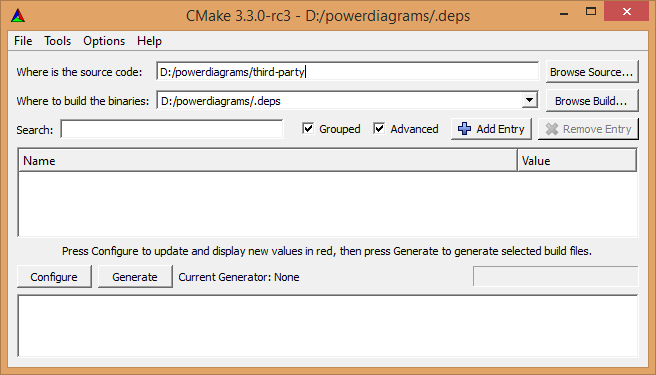
\includegraphics[width=0.9\linewidth]{cmake_1.png}
    \caption{The \src{third-party} directory contains a CMake script which downloads and builds the libraries needed by the \var{powerdiagram} executable.
    Choose \src{.deps} as the destination folder to ensure that the second step will automatically find the dependencies.}
    \label{fig:cmake_1}
\end{figure}
\begin{figure}[p]
    \centering
    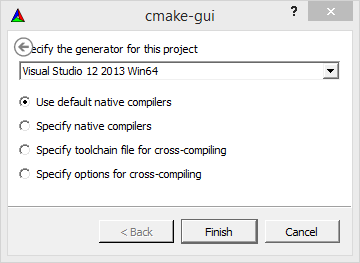
\includegraphics[width=0.45\linewidth]{cmake_2.png}
    \caption{After clicking the \enquote{Configure}-button, CMake prompts the user to choose a generator or toolchain.
    Visual Studio and MSVC are the most common toolchain on Windows.
    Both 32 and 64 bit builds are possible, but both libraries and the final program have to be built using the same generator.}
    \label{fig:cmake_2}
\end{figure}
\begin{figure}[p]
    \centering
    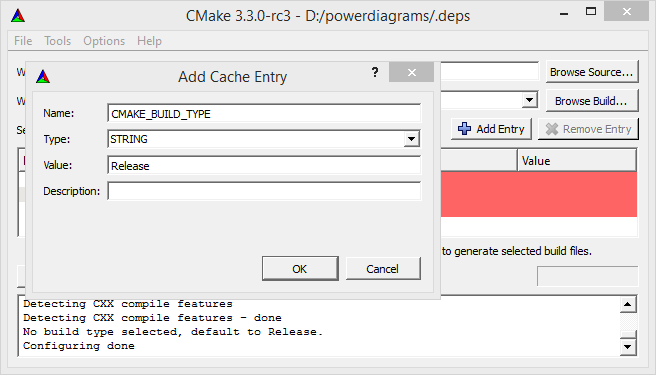
\includegraphics[width=0.9\linewidth]{cmake_3.png}
    \caption{To change the build type of the libraries from the default debug build to an optimized release build, add the according entry after the \enquote{Configure} step.}
    \label{fig:cmake_3}
\end{figure}
\begin{figure}[p]
    \centering
    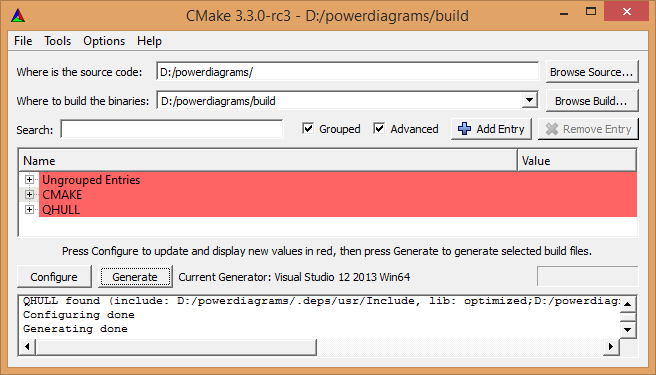
\includegraphics[width=0.9\linewidth]{cmake_4.png}
    \caption{To build the program executable, CMake has to be run again with the top level directory as the source folder.}
    \label{fig:cmake_4}
\end{figure}

To create a build on Windows, start with opening \var{cmake-gui} and creating the build files for the libraries.
\Cref{fig:cmake_1} shows the correct path to ensure that the later step will automatically find the dependencies.
The source CMake files can be found in \src{third-party}, while the binaries should be built into the folder \src{.deps} (including the period).

After choosing the folders, click the \enquote{Configure}-button and choose the desired generator as shown in \cref{fig:cmake_2}.
CMake checks whether the compiler works correctly and searches for correct paths.
By default, the libraries will be built with debug information.
If this is not desired (e.g. for an optimized build), change the \var{CMAKE\_BUILD\_TYPE} variable as shown in \cref{fig:cmake_3}.

After pressing the \enquote{Generate}-button, \src{.deps} should contain a Visual Studio solution file.
Open the solution with Visual Studio and start a build process, ignoring the build type options.
Visual Studio will download the source files and compile the libraries, installing them into the \src{.deps} folder.
This concludes the first step.

\begin{figure}[tb]
    \centering
    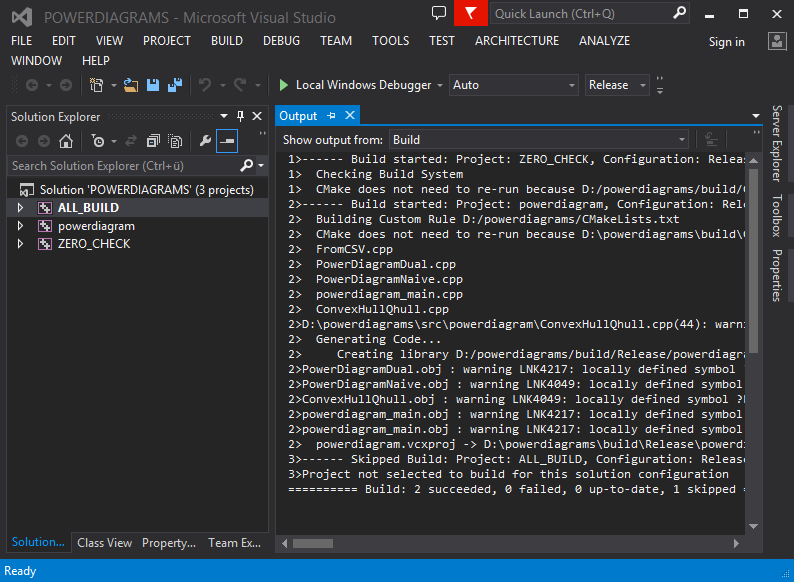
\includegraphics[width=0.9\linewidth]{cmake_5.png}
    \caption{The Visual Studio solution created by CMake for the program can be used to build the code in both debug and release mode.
    CMake found the correct paths for all libraries and configured Visual Studio accordingly.
    The solution explorer shows the \var{powerdiagram} executable which contains the source files which can be edited and debugged as usual.}
    \label{fig:cmake_4}
\end{figure}
Open a new \var{cmake-gui} and prepare the second step as shown in \cref{fig:cmake_4}.
The destination folder which will contain the final executable can be chosen freely.
After clicking \enquote{Configure} again, choose the same generator as before and click \enquote{Generate} --- changing the \var{CMAKE\_BUILD\_TYPE} here has no effect.
After this, the destination directory contains a Visual Studio solution which can be used to build the final program.

\section{Running the Program}
\label{sec:running_the_program}
The compiled program has a simple command line interface which allows the selection of power diagram sites, algorithms to be executed and output options.
The program includes a short documentation which can be viewed by invoking \var{./powerdiagram -help}.
The output of this invocation can be seen in \cref{lst:help}.
\begin{listing}[tb]
    \begin{minted}{shell}
Sample usage:
    ./powerdiagram [Options] <centers> <radii>
For a complete help, use options --help or --helpfull.

  Flags from (...)/powerdiagram/ConvexHullQhull.cpp:
    -qhullout (Output string for Qhull (e.g. "f i s"))
        type: string default: ""

  Flags from (...)/powerdiagram_main.cpp:
    -draw (Output Information needed to draw the Diagram)
        type: bool default: false
    -dual (Run the Dual Algorithm) type: bool default: true
    -naive (Run the Naive Algorithm) type: bool default: false
    -verbose (Verbose output) type: bool default: false
    \end{minted}
    \caption{The output of running \var{./powerdiagram -help}.}
    \label{lst:help}
\end{listing}

This section shows how to use the program to create a visualization of a two-dimensional power diagram in the \LaTeX-package tikz with \cref{fig:garage} as an example.
The first step is to choose the sphere centers and radii.
They are defined in two different text files where each line defines a site.
While the file defining the radii contains one number per line, the different entries of the vectors of the sphere centers are separated with commas, examples of which can be found in the \src{examples} folder.
A $d$ dimensional input must contain at least $(d+1)$ linearly independent sphere centers.
The files corresponding to \cref{fig:garage} are called \src{garage\_sites.csv} for the centers and \src{garage\_gamma.csv} for the radii.

\begin{listing}[tb]
    \begin{minted}{shell}
# Manual invocation
$ ./powerdiagram -draw garage_sites.csv garage_gamma.csv > /tmp/intrmdt
$ util/tikz.py /tmp/intermdt
# Using the Makefile
$ make TIKZ_OUT=1 garage
    \end{minted}
    \caption{To create a tikz picture from sphere centers and radii defined in text files, the \var{./powerdiagram -draw} parameter can be used.
        If the program is invoked with this parameter, it outputs a easily parseable format describing vertices and edges of a power diagram, which gets saved to a temporary file.
        This output is then parsed by a Python script which in turn creates a tikz picture.
        The Makefile mentioned in \cref{sub:linux} can also generate tikz output.}
    \label{lst:createtikz}
\end{listing}
\begin{listing}[tb]
    \begin{minted}{Python}
# Spheres
s1 2 3 1
s2 5 0 1
s3 -2  0  3
s4 2 0 2
s5 4 2 1

# Vertices
p1 0.625     2
p2    4 0.75
p3 2.75    2

# Internal Edges
ei p1 p3 s1 s4
ei p2 p3 s4 s5

# External Edges
ee p1 s1 s3 d-0.6  0.8
ee p1 s3 s4 d 0 -1
ee p2 s2 s4 d-0 -1
ee p2 s2 s5 d0.894427 0.447214
ee p3 s1 s5 d0.447214 0.894427
    \end{minted}
    \caption{The intermediate output format generated by \var{./powerdiagram -draw}.
    The output first enumerates both the spheres and vertices.
    Every internal edge can be defined as the connection of two of the vertices, while the external edges are defined as a point and a normalized direction of the ray.
    The additional annotations of the edge describe to which cells of spheres the edge is incident.}
    \label{lst:intermediate}
\end{listing}
Creating a tikz output is a two-step process.
The \CC executable itself cannot produce tikz but rather outputs a format which is easily parseable.
The file \src{util/tikz.py} contains a Python-script which converts this intermediate format to tikz output.
The commands that need to be executed can be found in \cref{lst:createtikz} with the intermediate output of the \CC program described in \cref{lst:intermediate}.
There is also a template in \src{util/template.tex} which can be used to quickly compile the output of the script files into a standalone image.

\clearpage
\printbibliography
\end{document}
